
\FloatBarrier
\section{Система Sprott A}  % {{{1
\label{atu:sect:spr_a}

\LinkRef{
  spr\_a: MKMM-2016
}

\subsection{Определение системы и анализ её динамики} %  % {{{2 _SPR_task

В своих работах J.C.~Sprott рассмотрел целое семейство динамических
систем, реализующих хаотическое поведение, обозначив их латинскими буквами
от ``A'' до ``S''~\cite{sprott_212,sprott_strange_attr}. Особое место среди них
занимает система, обозначаемая как ``Sprott A''. Отличительной особенностью
этой системы является отсутствие положений равновесия, что делает
невозможным применение многих известных методов анализа, основанных на
каком-либо разложении в окрестностях точек равновесия. Соответствующая ей
система уравнений имеет вид:
%
\begin{equation}
  \begin{cases}
    \dot{x} =  y, \\
    \dot{y} = -x + yz, \\
    \dot{z} =  1 - y^2.
  \end{cases}
  \label{atu:eq:spr_a_orig}
\end{equation}


В исходном виде система (\ref{atu:eq:spr_a_orig}) имеет фиксированные значения параметров.
Не изменяя структуры системы, можно ввести 5 параметров, влияющие на её динамку.
Поскольку целью данной работы является определение возможности применения
различных критериев идентификации параметров
хаотических объектов, а также свойств методов идентификации, то для данной системы
рассмотрим только один параметр --- $c_{x_y} $. Система принимает следующий вид:
%
\begin{equation}
  \begin{cases}
    \dot{x} =  c_{x_y} y, \\
    \dot{y} = -x + yz, \\
    \dot{z} =  1 - y^2.
  \end{cases}
  \label{atu:eq:spr_a}
\end{equation}

В таком виде система, при изменении $c_{x_y} $
в достаточно широком диапазоне может демонстрировать как
сложно-периодическое (рис.~\ref{atu:f:spr_a_p_0372}), так и преимущественно, хаотическое
поведение (рис.~\ref{atu:f:spr_a_p_0610}).

\begin{figure}[htb!]
\centerline{
  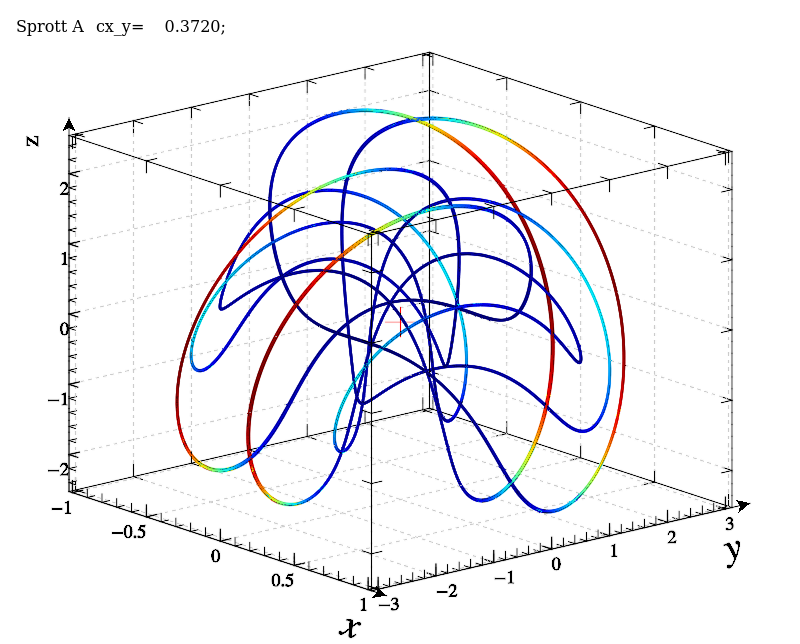
\includegraphics[width=0.49\textwidth]{p/cha/spr_a/sprott_a-p_xyz_cx_y=0x372.png}
  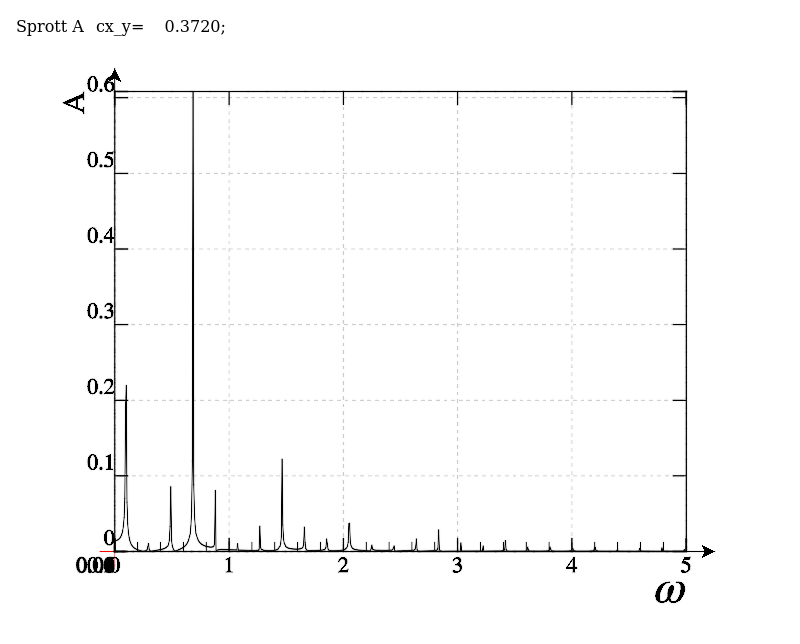
\includegraphics[width=0.49\textwidth]{p/cha/spr_a/sprott_a_f-p_f_cx_y=0x372.png}
}
\caption{Аттрактор и спектр системы (\ref{atu:eq:spr_a}) при $ c_{x_y} =0.372 $.
  Сложно-периодический режим.
}
\label{atu:f:spr_a_p_0372}
\end{figure}

При этом, в диапазоне $c_{x_y} \in [0.1 ; 0.7] $
наблюдаются перестройки структуры аттрактора, а при относительно больших
значениях данного параметра аттрактор представляет собой полый тор.

\begin{figure}[htb!]
\centerline{
  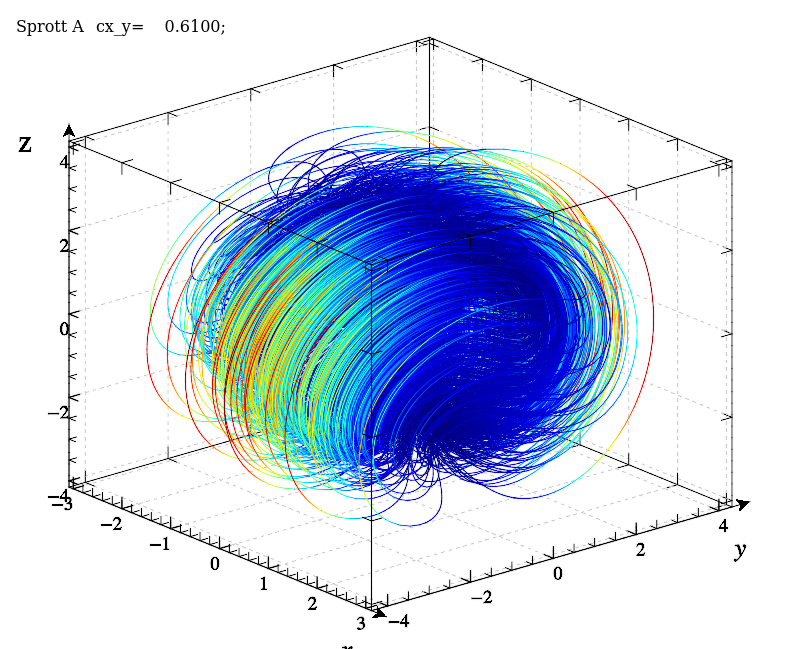
\includegraphics[width=0.49\textwidth]{p/cha/spr_a/sprott_a-p_xyz_cx_y=0x610.png}
  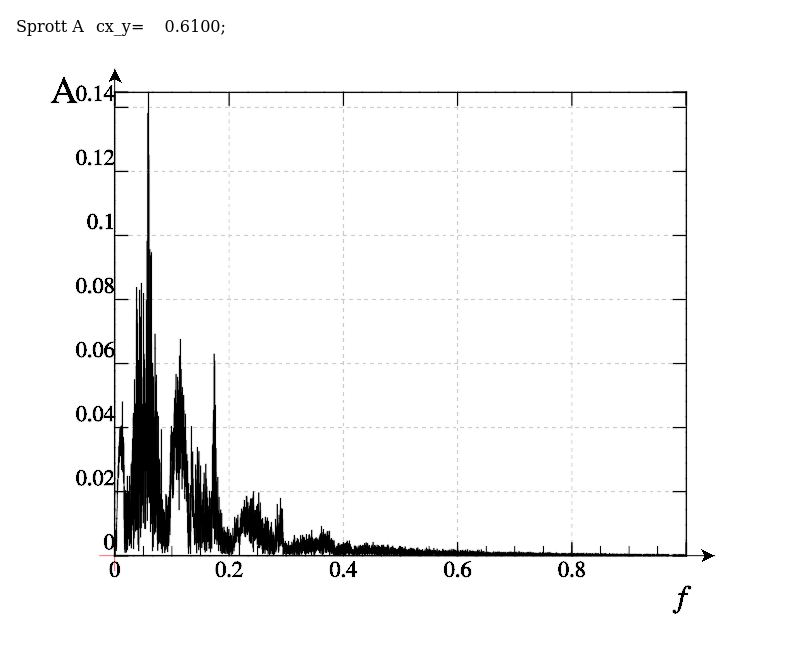
\includegraphics[width=0.49\textwidth]{p/cha/spr_a/sprott_a_f-p_f_cx_y=0x610.png}
}
\caption{Аттрактор и спектр системы (\ref{atu:eq:spr_a}) при $ c_{x_y} =0.610 $.
  Хаотический режим
}
\label{atu:f:spr_a_p_0610}
\end{figure}




Важной особенностью поведения этой системы является то, что при $ c_{x_y} \ge 1 $
в спектре системы имеются очень ограниченные участки сплошного спектра~(рис.~\ref{atu:f:spr_a_p_1000}).
При этом, как и для получения корректного спектра, так и для обнаружения ``разбегания'' траекторий
необходимо моделирование системы на протяжении достаточно длительного
(по сравнению с многими схожими системами) модельного времени.

\begin{figure}[htb!]
\centerline{
  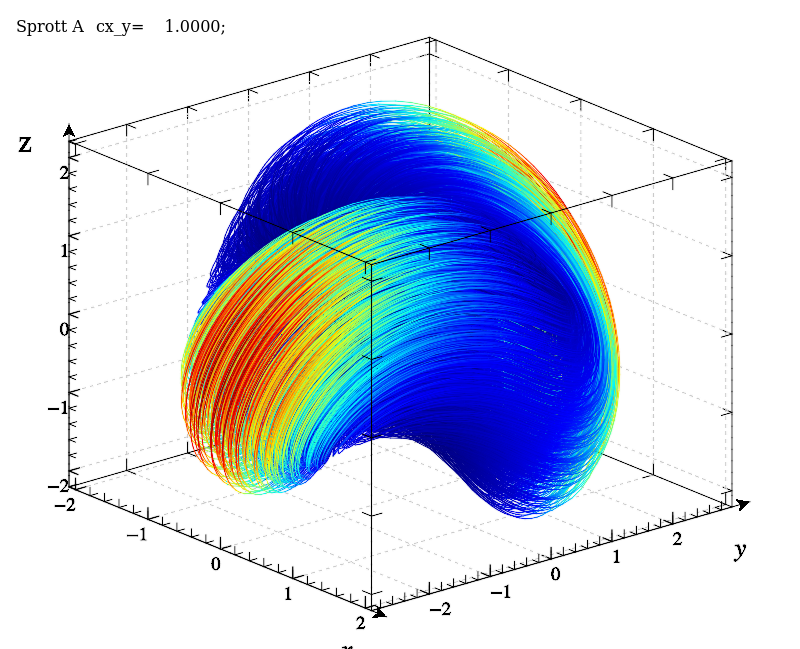
\includegraphics[width=0.49\textwidth]{p/cha/spr_a/sprott_a-p_xyz_cx_y=1x000.png}
  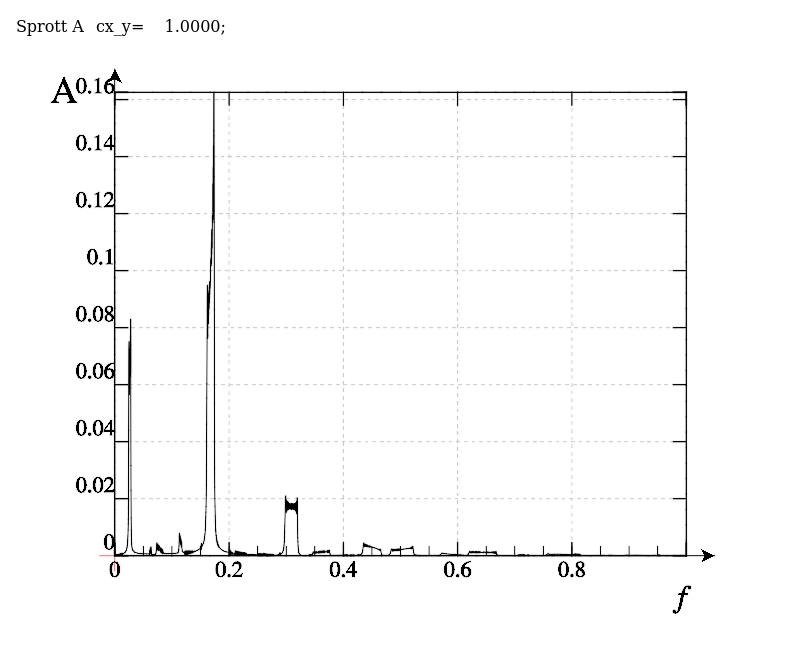
\includegraphics[width=0.49\textwidth]{p/cha/spr_a/sprott_a_f-p_f_cx_y=1x000.png}
}
\caption{Аттрактор и спектр системы (\ref{atu:eq:spr_a}) при $ c_{x_y} =1.0 $.
}
\label{atu:f:spr_a_p_1000}
\end{figure}

% }}}2


\subsection{Анализ и выбор критериев}  % {{{2

В первую очередь, на аналогии с системой Лоренца,
проверим возможность применения энергетических критериев,
так как существуют реальные физические системы,
для моделирования которых применяется система~~(\ref{atu:eq:spr_a_orig}).

Рассмотрим зависимости $q_{*}(c_{x_y}) $ (рис.~\ref{atu:f:spr_a_q})
для системы (\ref{atu:eq:spr_a}). Анализ этих зависимостей
даёт практически однозначный ответ о возможном виде критерия --- $q_{x^2}$.
Второй кандидат --- $q_{x}$ --- обладает меньшей линейностью.
Также следует отметить, что
значения критериев, в которые не входит $x$, практически не зависят от $c_{x_y}$,
а вид критериев $q_{xy}$ и $q_{xz}$ ничем не лучше, чем у $q_{x}$.
Таким образом, систему идентификации будем строить, используя критерий~$q_{x^2}$~\cite{atu_kher2016}.

\begin{figure}[htb!]
\centerline{
  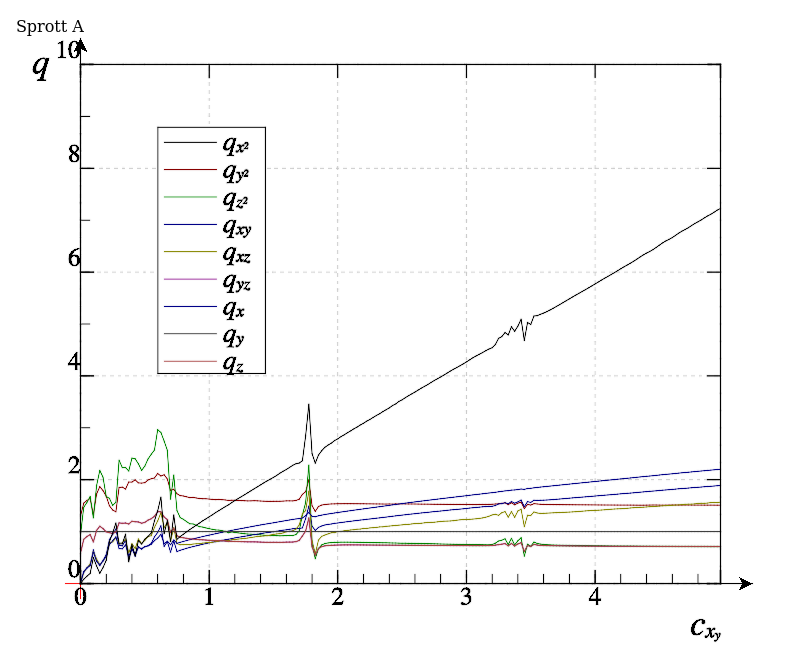
\includegraphics[width=0.60\textwidth]{p/cha/spr_a/sprott_a_q-p_c_x_y.png}
}
\caption{Зависимости $q_{*}(c_{x_y})$ для системы (\ref{atu:eq:spr_a}) }
\label{atu:f:spr_a_q}
\end{figure}

Нельзя не отметить, что в начальной области
$q_{x^2}(c_{x_y}) $, а именно там, где происходят постоянные
перестройки структуры аттрактора, ни один из рассматриваемых критериев
не имеет достаточной монотонности, что не даёт гарантии
построения работоспособной системы идентификации.
Для работы в этой области, скорее всего, требуется синтез специальных критериев.
Также, в окрестности точки $c_{x_y}=1.775$ аттрактор также резко изменяет свою структуру.
Так как это достаточно узкая окрестность,
то можно предположить, что мультиагентная система идентификации
не окажется неработоспособной в этой области, просто вырастет
ошибка идентификации.

Для проведения идентификации было выбрано два семейства методов:
ql3rlWvnAAW.$q_{x^2}$ и
Fq3rlFvnAAF.$q_{x^2}$.

Рассмотрим зависимости, определяющие
требуемые интервалы усреднения критериев идентификации
--- $ \sigma_q(\tau_q) $
или же  $ \sigma_q(a_q) $ --- соотношение между
временем оценивания $\tau_q$ и среднеквадратичной
ошибкой измерения критерия.

Для моделирования непосредственных погрешностей измерения величины
$x(t)$ использовался шум с нормальным распределением
и параметрами $\sigma_w=0.1$ и $\tau_w=0.05$.
Для оценивания требуемой зависимости, для каждого
значения $\tau_q$ из заданного диапазона
проводилось $N=200$ процессов моделирования динамики системы,
и в случайный момент (достаточно далеко отстоящий от точки $t=0$ для исключения краевых эффектов)
проводилось измерение и запоминание выбранного критерия.
Так же, как для системы Лоренца,
для усреднения величины $q$ использовалось 2 метода:
экспоненциального сглаживания, вида (\ref{atu:eq:qlin}), и скользящее среднее.
Полученные зависимости,  представлены на
рис.~\ref{atu:f:spr_a_qx2_tau}.


\begin{figure}[htb!]
\begin{center}
  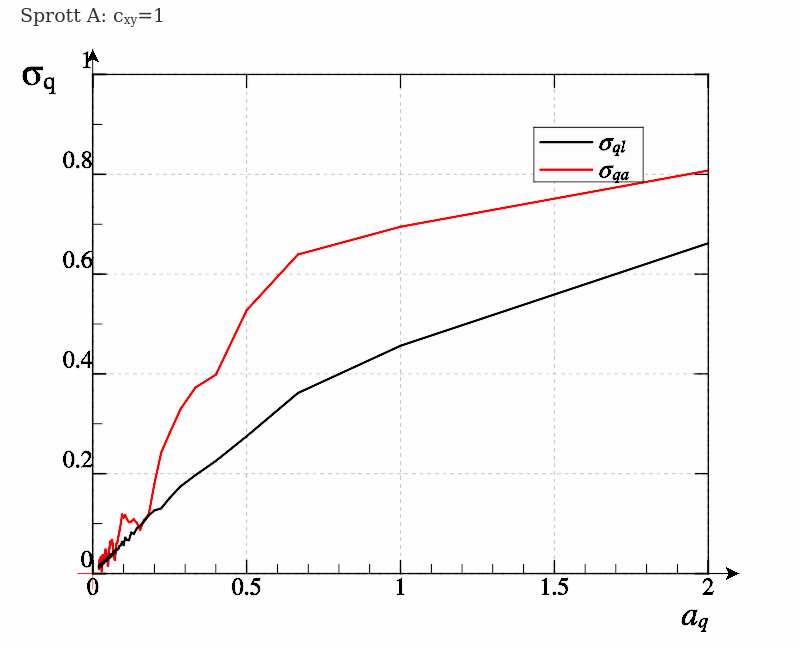
\includegraphics[width=0.49\textwidth]{p/cha/spr_a/sprott_a_qx2_tau-p_aq_sd.png}
  \hfill
  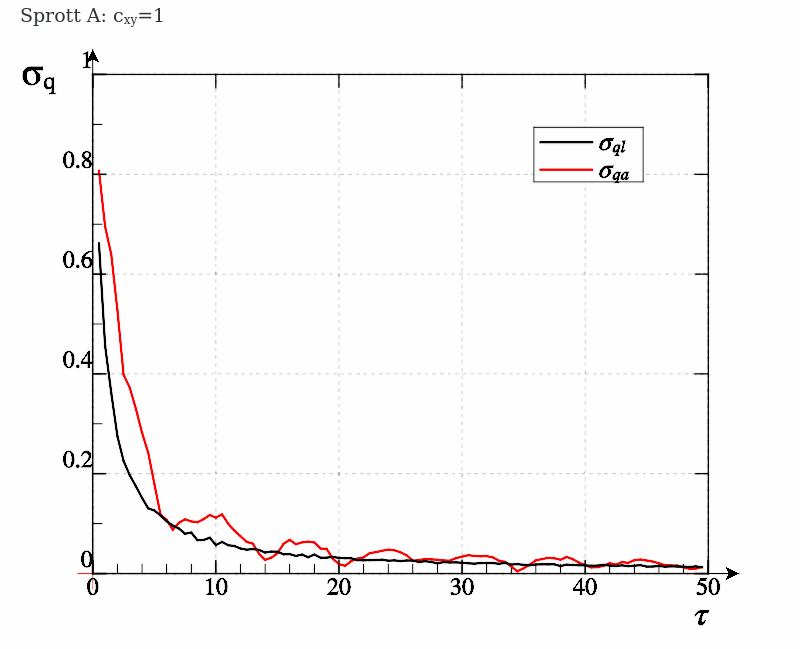
\includegraphics[width=0.49\textwidth]{p/cha/spr_a/sprott_a_qx2_tau-p_tau_sd.png}
\end{center}
  \caption{Зависимости $\sigma_{q}(a_q)$ и $\sigma_{q}(\tau_q)$ для системы Sprott A, критерий  $q_{x^2}$}
\label{atu:f:spr_a_qx2_tau}
\end{figure}

Вид этих зависимостей практически не отличается
от аналогичных для системы Лоренца (рис.\ref{atu:f:lor_qx2_tau}).
Совершенно аналогично, скользящее среднее в данных условиях
не даёт никаких преимуществ и не будет использоваться далее.

% }}}2


\subsection{Тестовая задача идентификации для системы Sprott A}   % {{{2

В соответствии с полученными данными, и используя
предложения~(\ref{atu:eq:po_t_sign}) и~(\ref{atu:eq:po_t_sin}),
определим тестовую задачу следующим образом:
\[
  c_{x_y}(t) \equiv p_o(t) \in (0, 5],
\]
%
\begin{equation}
  p_o(t) = p_0 +  U_{p} \sign \sin( \omega_{p} t ),
  \label{atu:eq:spr_a_po_t_sign}
\end{equation}
%
%
\begin{equation}
  p_o(t) = p_0 +  U_{p} \sin( \omega_{p} t ),
  \label{atu:eq:spr_a_po_t_sin}
\end{equation}
%
где:
$p_0 = 2.8$, $U_p=1.9$, $\omega_p=0.0104719755$.

На рис.~\ref{atu:f:spr_a_id_ql3rlWvnAAW_q_x2_sign} представлены результаты
моделирования процесса идентификации
группой методов ql3rlWvnAAW.$q_{x^2}$. Аналогично системе Лоренца, на левом графике представлена
динамика перемещения каждой из подвижных моделей,
а на правом --- 8 способов определения $p_\mathrm{id}(t)$.

\begin{figure}[htb!]
  \centerline{
    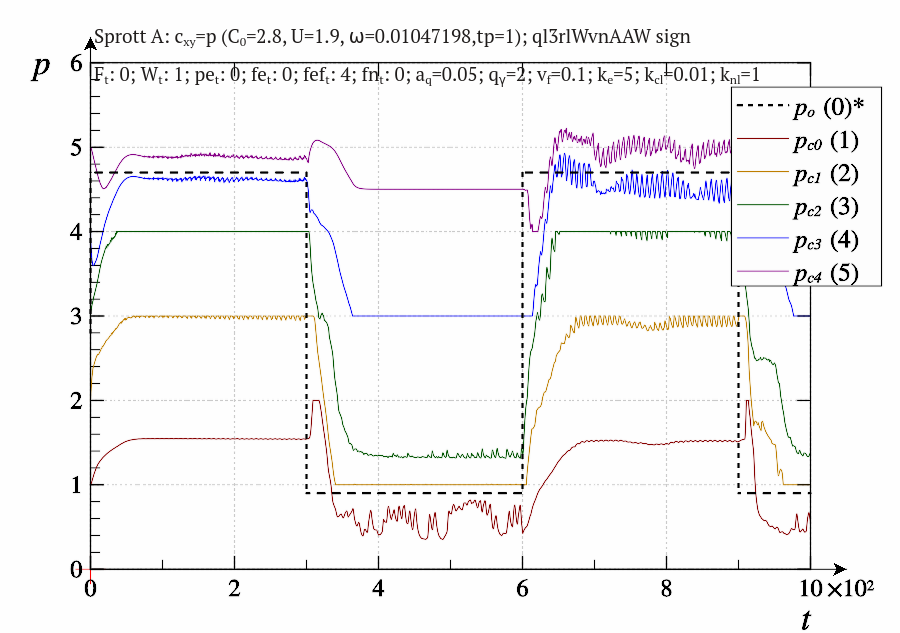
\includegraphics[width=0.49\textwidth]{p/cha/spr_a/ql3rlWvnAAW_x2/sprott_a_id-p_t_pi_ql3rlWvnAAW_sign.png}
    \hfill
    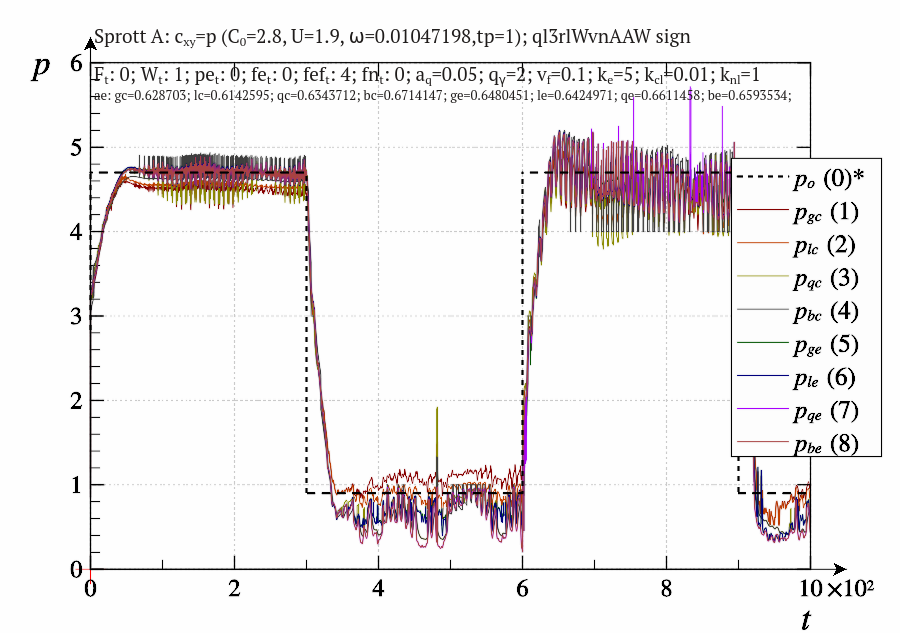
\includegraphics[width=0.49\textwidth]{p/cha/spr_a/ql3rlWvnAAW_x2/sprott_a_id-p_t_p_ql3rlWvnAAW_sign.png}
  }
  \caption{Процесс идентификации параметра ``$c_{x_y}$'' системы Sprott A группой методов ql3rlWvnAAW.$q_{x^2}$ при условии~(\ref{atu:eq:spr_a_po_t_sign})}
  \label{atu:f:spr_a_id_ql3rlWvnAAW_q_x2_sign}
\end{figure}

В первую очередь, следует отметить различие между процессами
идентификации этим методом данной системы и система Лоренца.
Зависимость $p_{be}(t)$, в данном случае демонстрирует
высокий уровень колебаний, и следовательно,
худшие результаты поиска. При этом,
остальные подходы к определению $p_\mathrm{id}$
демонстрируют схожие между собой результаты.
Также следует отметить, что на третьем полупериоде уровень колебаний заметно выше,
чем на первом. Анализ значений критерия показывает, что это обусловлено
реакцией объекта на скачкообразное изменение параметра.
%$\overline{e}_{bm}=1.41$
%$\overline{e}_{ba}=1.49$.



На рис.~\ref{atu:f:spr_a_id_ql3rlWvnAAW_q_x2_sin} представлены аналогичные результаты,
но при условии плавного изменение значения $p_o(t)$. Также очевидно, что
как абсолютные, так и относительные значения ошибок идентификации в данном случае несколько
меньше, при сохранении общей картины.
%$\overline{e}_{bm}=0.91$
%и
%$\overline{e}_{ba}=0.84$.

\begin{figure}[htb!]
  \centerline{
    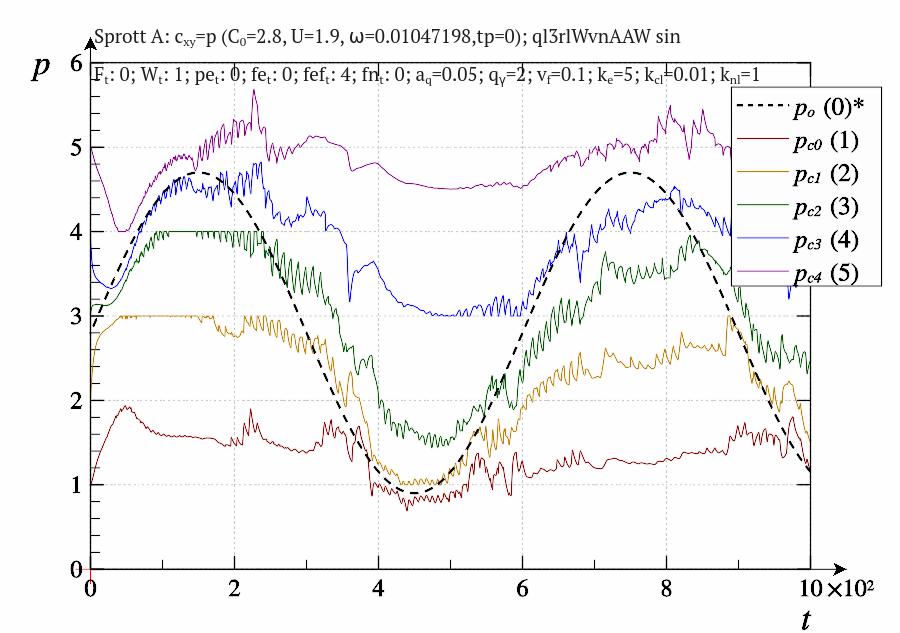
\includegraphics[width=0.49\textwidth]{p/cha/spr_a/ql3rlWvnAAW_x2/sprott_a_id-p_t_pi_ql3rlWvnAAW_sin.png}
    \hfill
    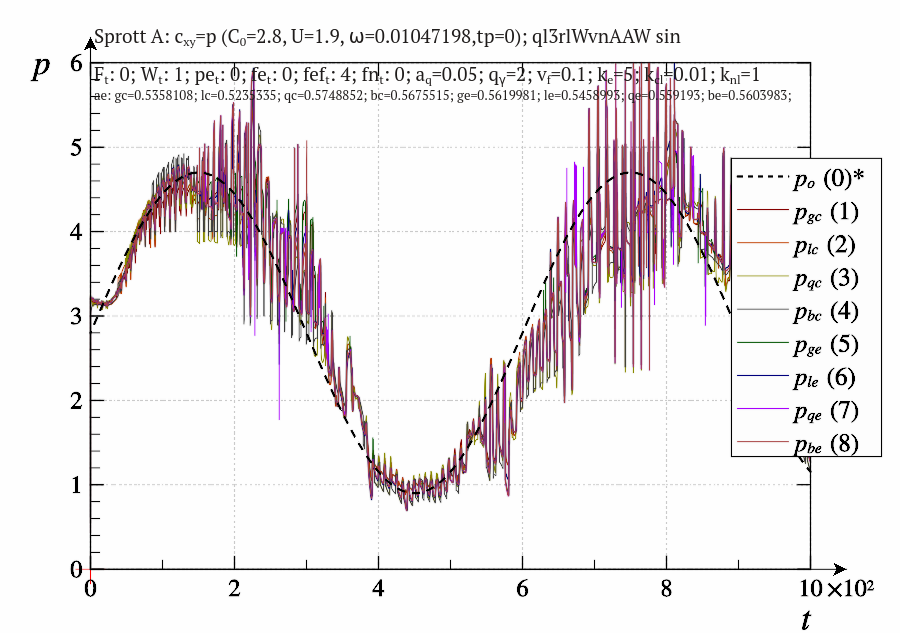
\includegraphics[width=0.49\textwidth]{p/cha/spr_a/ql3rlWvnAAW_x2/sprott_a_id-p_t_p_ql3rlWvnAAW_sin.png}
  }
  \caption{Процесс идентификации параметра ``$c_{x_y}$'' системы Sprott A группой методов ql3rlWvnAAW.$q_{x^2}$ при условии~(\ref{atu:eq:spr_a_po_t_sin})}
  \label{atu:f:spr_a_id_ql3rlWvnAAW_q_x2_sin}
\end{figure}

Для проверки равномерности ошибки идентификации на всём рабочем диапазоне параметра
была проведена идентификация, при которой значение параметра
плавно пробегало весь диапазон, т.е. использовалось условие (\ref{atu:eq:po_t_ramp}).
Результаты моделирования приведены на рис.~\ref{atu:f:spr_a_id_ql3rlWvnAAW_q_x2_ramp}.
Эти результаты позволяют сделать вывод о том, что в верхней части диапазона
наблюдается плавный рост ошибки идентификации, что не следует из
вида критерия. Однако, отмеченные локальные возмущения критерия
не привели к заметным отклонениям.


\begin{figure}[htb!]
  \centerline{
    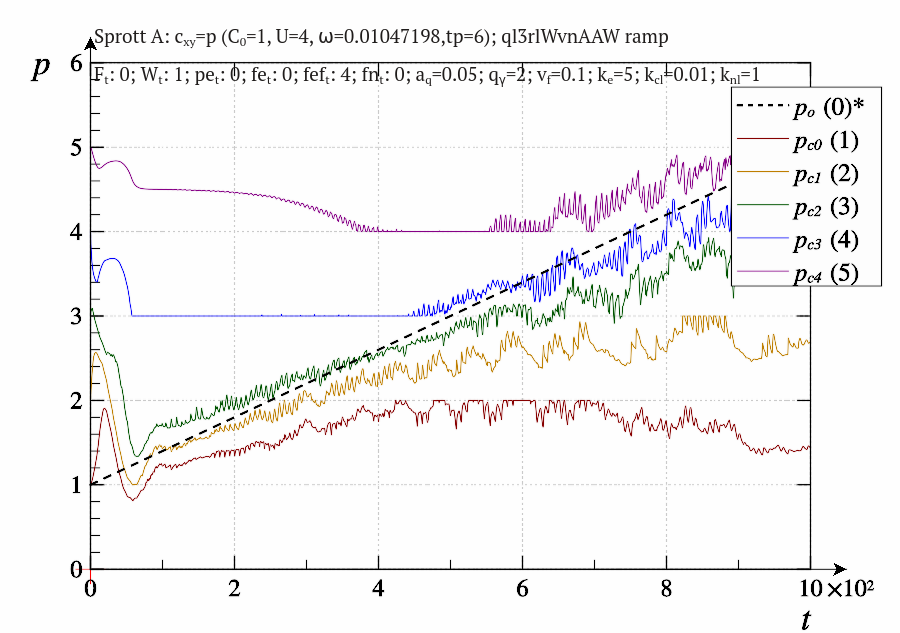
\includegraphics[width=0.49\textwidth]{p/cha/spr_a/ql3rlWvnAAW_x2/sprott_a_id-p_t_pi_ql3rlWvnAAW_ramp.png}
    \hfill
    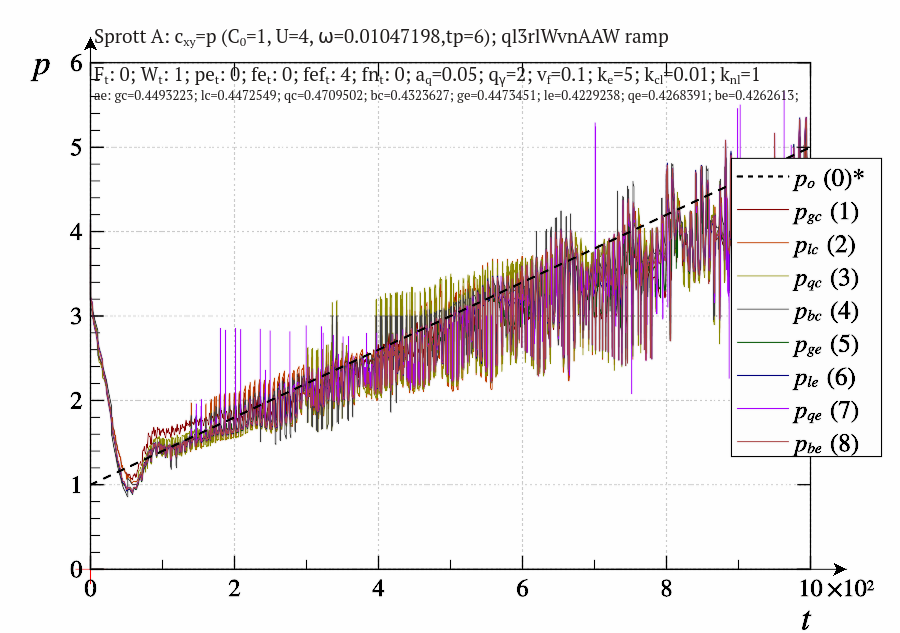
\includegraphics[width=0.49\textwidth]{p/cha/spr_a/ql3rlWvnAAW_x2/sprott_a_id-p_t_p_ql3rlWvnAAW_ramp.png}
  }
  \caption{Процесс идентификации параметра ``$c_{x_y}$'' системы Sprott A группой методов ql3rlWvnAAW.$q_{x^2}$ при условии~(\ref{atu:eq:po_t_ramp})}
  \label{atu:f:spr_a_id_ql3rlWvnAAW_q_x2_ramp}
\end{figure}

На рис.~\ref{atu:f:spr_a_id_Fq3rlFvnAAF_q_x2_sign} представлены результаты идентификации
группой методов Fq3rlFvnAAF.$q_{x^2}$.
Уровень ошибок идентификации имеет практически одинаковые значения
по сравнению с группой методов ql3rlWvnAAW. При этом
заметно больший уровень ошибки наблюдается при использовании
метода $p_{gc}$ в процессе работы координатора поиска.
% $\overline{e}_{bm}=1.71$


\begin{figure}[htb!]
  \centerline{
    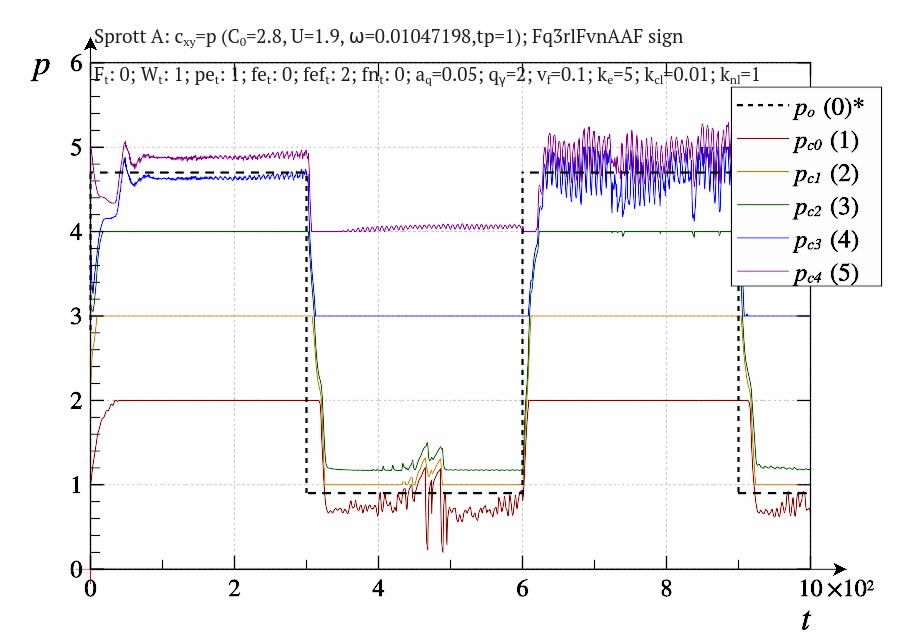
\includegraphics[width=0.49\textwidth]{p/cha/spr_a/Fq3rlFvnAAF_x2/sprott_a_id-p_t_pi_Fq3rlFvnAAF_sign.png}
    \hfill
    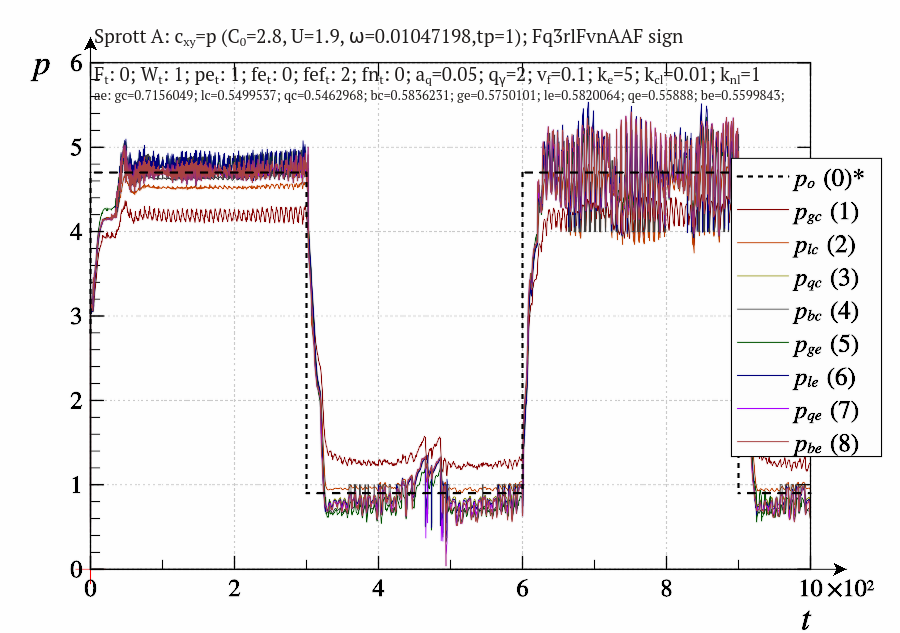
\includegraphics[width=0.49\textwidth]{p/cha/spr_a/Fq3rlFvnAAF_x2/sprott_a_id-p_t_p_Fq3rlFvnAAF_sign.png}
  }
  \caption{Процесс идентификации параметра ``$c_{x_y}$'' системы Sprott A группой методов Fq3rlFvnAAF.$q_{x^2}$ при условии~(\ref{atu:eq:spr_a_po_t_sign})}
  \label{atu:f:spr_a_id_Fq3rlFvnAAF_q_x2_sign}
\end{figure}

На рис.~\ref{atu:f:spr_a_id_Fq3rlFvnAAF_q_x2_sin} представлены аналогичные результаты,
но при условии плавного изменение значения параметра объекта. Очевидно, что
как абсолютные, так и относительные значения ошибок идентификации в данном случае заметно
меньше, при сохранении общей картины.
%$\overline{e}_{bm}=0.87$

\begin{figure}[htb!]
  \centerline{
    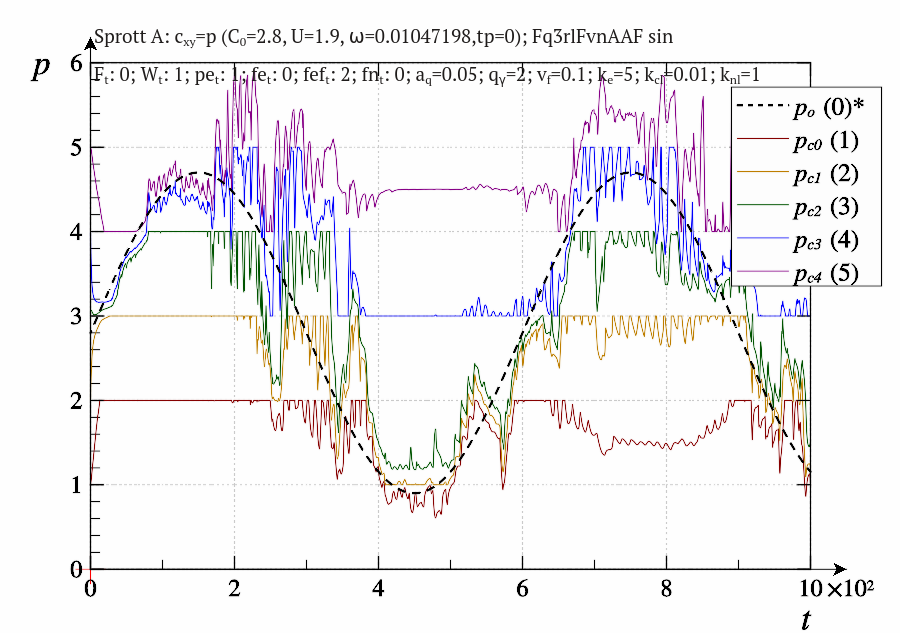
\includegraphics[width=0.49\textwidth]{p/cha/spr_a/Fq3rlFvnAAF_x2/sprott_a_id-p_t_pi_Fq3rlFvnAAF_sin.png}
    \hfill
    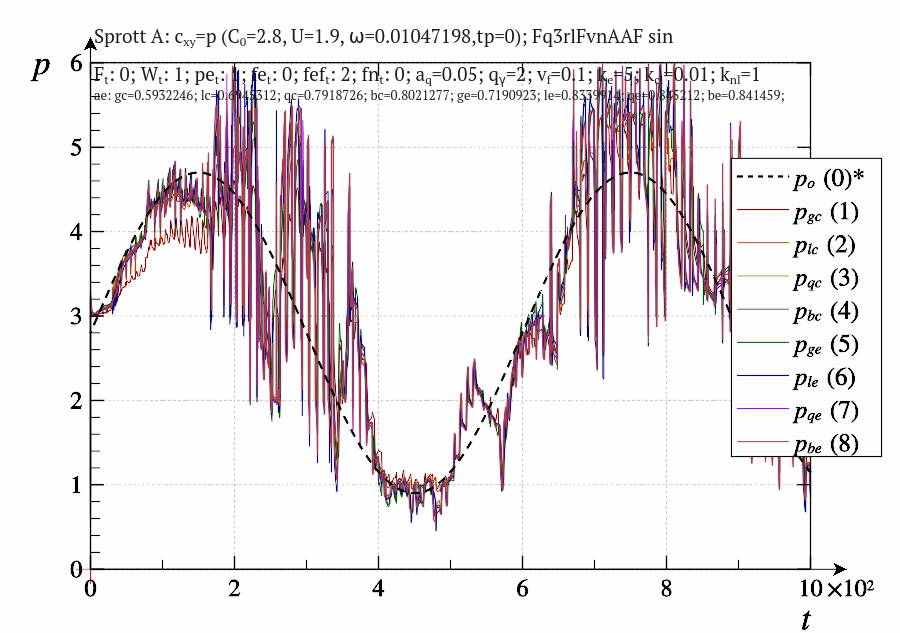
\includegraphics[width=0.49\textwidth]{p/cha/spr_a/Fq3rlFvnAAF_x2/sprott_a_id-p_t_p_Fq3rlFvnAAF_sin.png}
  }
  \caption{Процесс идентификации параметра ``$c_{x_y}$'' системы Sprott A группой методов Fq3rlFvnAAF.$q_{x^2}$ при условии~(\ref{atu:eq:spr_a_po_t_sin})}
  \label{atu:f:spr_a_id_Fq3rlFvnAAF_q_x2_sin}
\end{figure}

Результаты проверки равномерности ошибки идентификации на всём рабочем диапазоне параметра
приведены на рис.~\ref{atu:f:spr_a_id_Fq3rlFvnAAF_q_x2_ramp}.


\begin{figure}[htb!]
  \centerline{
    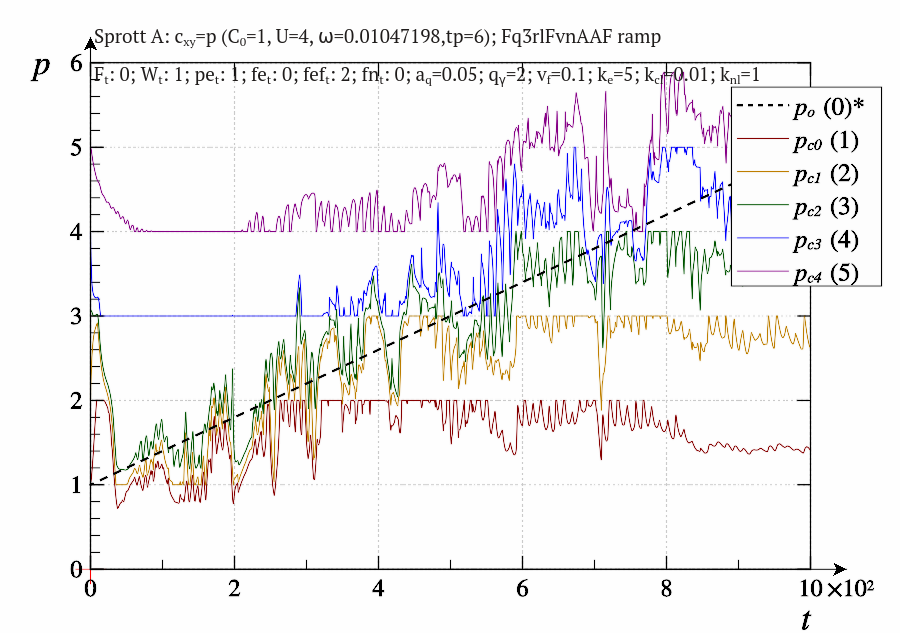
\includegraphics[width=0.49\textwidth]{p/cha/spr_a/Fq3rlFvnAAF_x2/sprott_a_id-p_t_pi_Fq3rlFvnAAF_ramp.png}
    \hfill
    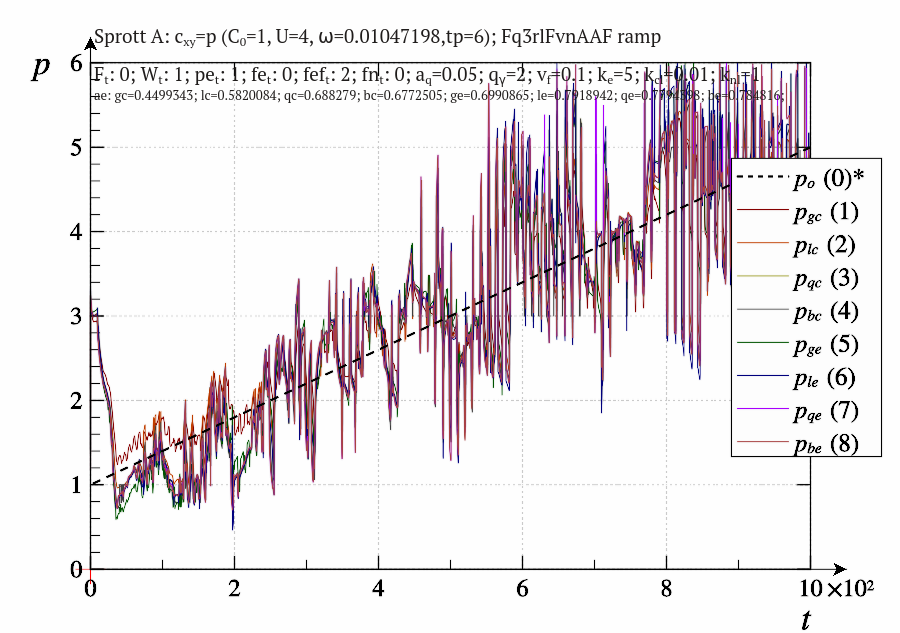
\includegraphics[width=0.49\textwidth]{p/cha/spr_a/Fq3rlFvnAAF_x2/sprott_a_id-p_t_p_Fq3rlFvnAAF_ramp.png}
  }
    \caption{Процесс идентификации параметра ``$c_{x_y}$'' системы Sprott A группой методов Fq3rlFvnAAF.$q_{x^2}$ при условии~(\ref{atu:eq:po_t_ramp})}
  \label{atu:f:spr_a_id_Fq3rlFvnAAF_q_x2_ramp}
\end{figure}

Общий уровень колебаний на этом графике не даёт возможности достаточно корректно оценить
равномерность уровня ошибки при изменении значения параметра. Однако,
в данном вычислительном эксперименте сохраняется работоспособность системы идентификации,
а группа методов Fq3rlFvnAAF в целом немного уступает группе ql3rlWvnAAW.


% }}}2


\subsection{Влияние параметров системы идентификации на ошибку идентификации для системы Sprott A}  % {{{2


Рассмотрим влияние параметров системы идентификации на
ошибки идентификации.

Первый параметр ---
$a_q$, определяющий характерное время усреднения критерия.

На рис.~\ref{atu:f:spr_a_a_q_ql3rlWvnAAW_q_x2} представлены зависимости
$\overline{e}(a_q)$ при применении метода ql3rlWvnAAW.$q_{x^2}$.
Вид зависимостей аналогичен таковым, полученным для идентификации
системы Лоренца~\cite{atu_kher2015}, и определяется он теми же факторами,
то есть положение экстремума определяется балансом между
динамическими свойствами самой системы и динамикой
изменения параметра.


\begin{figure}[htb!]
  \centerline{
    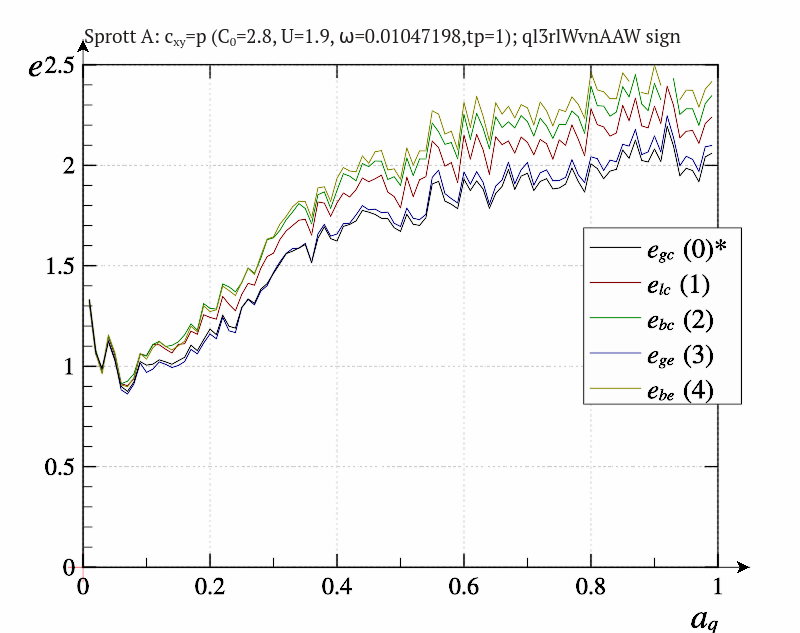
\includegraphics[width=0.49\textwidth]{p/cha/spr_a/ql3rlWvnAAW_x2/sprott_a_id-p_a_q_sign.png}
    \hfill
    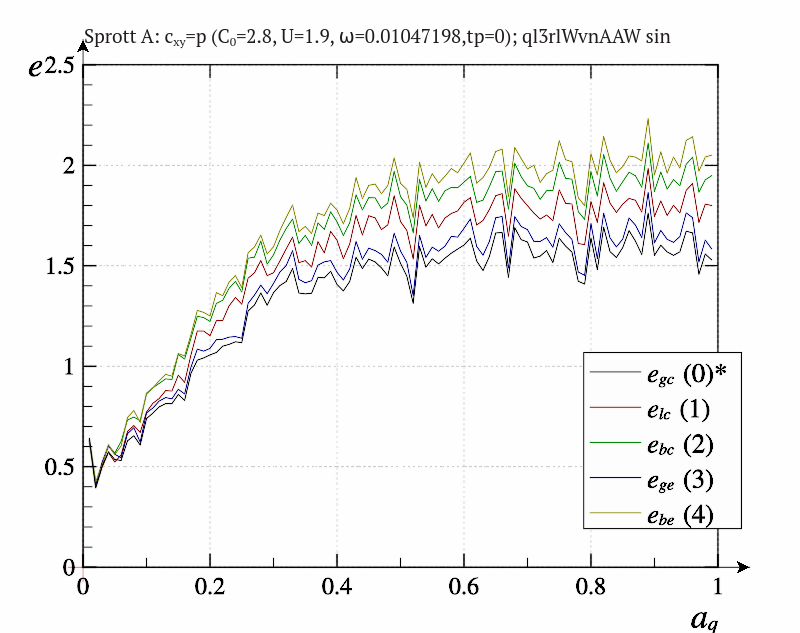
\includegraphics[width=0.49\textwidth]{p/cha/spr_a/ql3rlWvnAAW_x2/sprott_a_id-p_a_q_sin.png}
  }
  \caption{Зависимости $\overline{e}(a_q)$ при идентификации системы Sprott A группой методов ql3rlWvnAAW.$q_{x^2}$
   при~(\ref{atu:eq:spr_a_po_t_sign}) и (\ref{atu:eq:spr_a_po_t_sin})}
  \label{atu:f:spr_a_a_q_ql3rlWvnAAW_q_x2}
\end{figure}


На рис.~\ref{atu:f:spr_a_a_q_Fq3rlFvnAAF_q_x2} представлены зависимости
$\overline{e}(a_q)$ при применении метода Fq3rlFvnAAF.$q_{x^2}$.
И в этом случае получены результаты, не выбивающиеся из общего ряда.
Минимальные значения ошибок идентификации практически совпадают
с таковыми при применении предыдущего метода, а требуемое
время усреднения критерия немого больше. Несмотря на это,
при прочих равных данный метод обеспечивает несколько больший уровень колебания $p_\mathrm{id}$
в процессе поиска.


\begin{figure}[htb!]
  \centerline{
    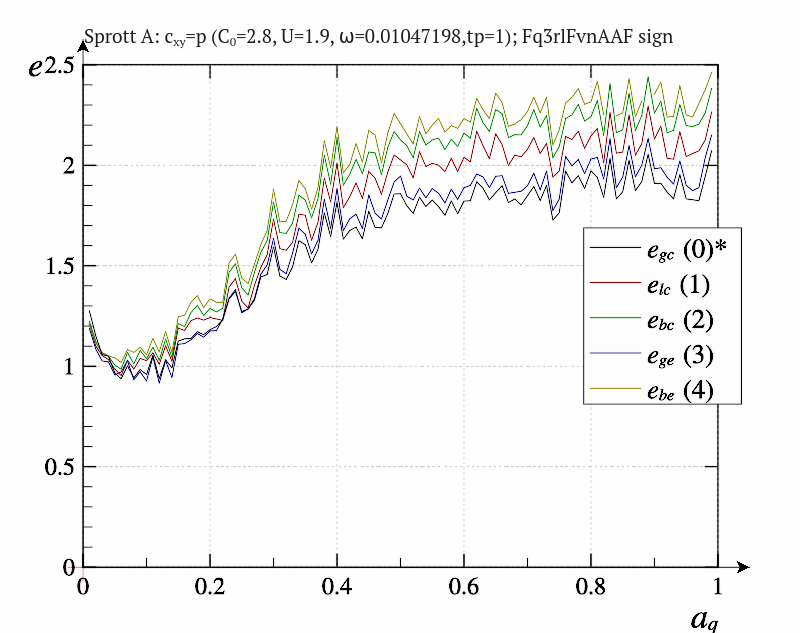
\includegraphics[width=0.49\textwidth]{p/cha/spr_a/Fq3rlFvnAAF_x2/sprott_a_id-p_a_q_sign.png}
    \hfill
    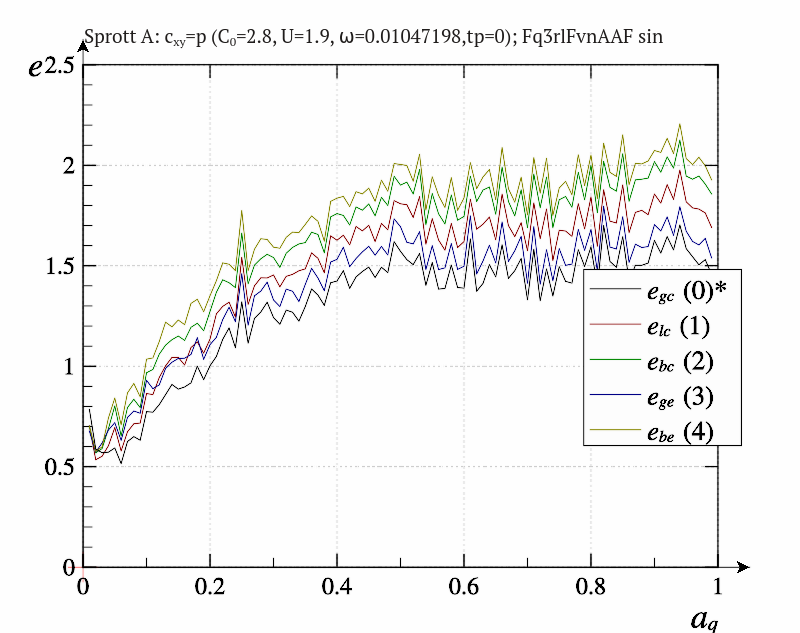
\includegraphics[width=0.49\textwidth]{p/cha/spr_a/Fq3rlFvnAAF_x2/sprott_a_id-p_a_q_sin.png}
  }
  \caption{Зависимости $\overline{e}(a_q)$ при идентификации системы Sprott A группой методов Fq3rlFvnAAF.$q_{x^2}$
   при~(\ref{atu:eq:spr_a_po_t_sign}) и (\ref{atu:eq:spr_a_po_t_sin})}
  \label{atu:f:spr_a_a_q_Fq3rlFvnAAF_q_x2}
\end{figure}

Следующий параметр --- $q_\gamma$ должен оказывать большее влияние на процессы идентификации,
использующие для оценки $p_e$ функцию качества.

На рис.~\ref{atu:f:spr_a_ql3rlWvnAAW_q_x2} представлены зависимости
$\overline{e}(q_\gamma)$ при применении группы методов ql3rlWvnAAW.$q_{x^2}$.
Рост ошибок идентификации при росте $q_\gamma < 2$
прогнозируем, при этом различные способы оценивания $p_\mathrm{id}$
дают практически неразличимые результаты.

\begin{figure}[htb!]
  \centerline{
    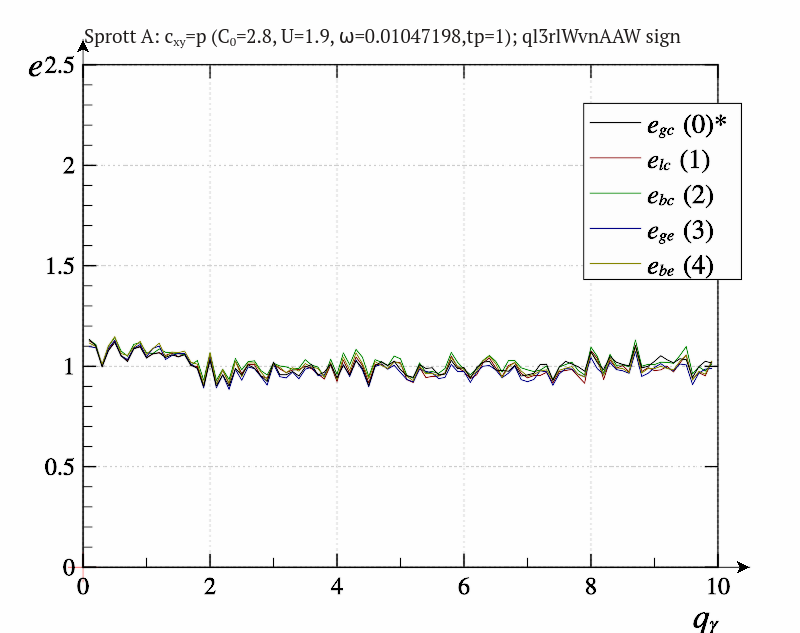
\includegraphics[width=0.49\textwidth]{p/cha/spr_a/ql3rlWvnAAW_x2/sprott_a_id-p_q_gamma_sign.png}
    \hfill
    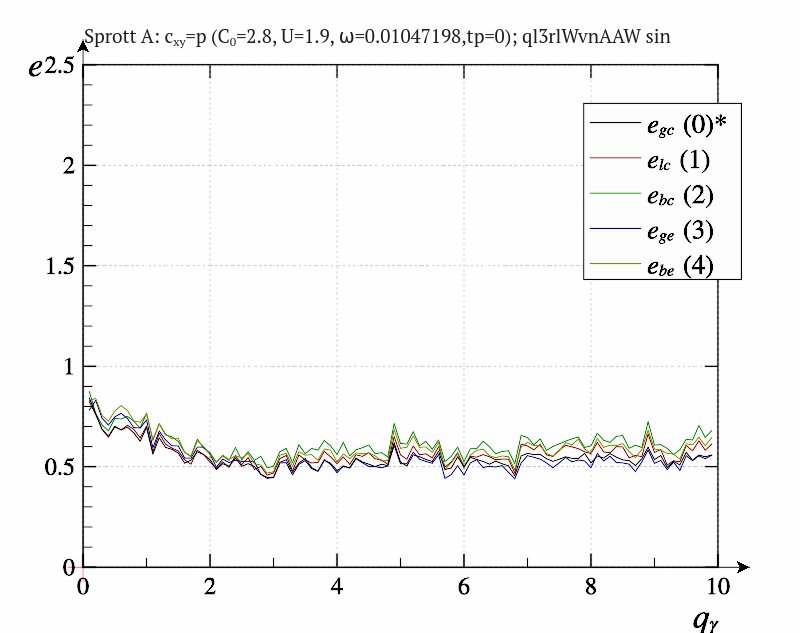
\includegraphics[width=0.49\textwidth]{p/cha/spr_a/ql3rlWvnAAW_x2/sprott_a_id-p_q_gamma_sin.png}
  }
  \caption{Зависимости $\overline{e}(q_\gamma)$ при идентификации системы Sprott A группой методов ql3rlWvnAAW.$q_{x^2}$
   при~(\ref{atu:eq:spr_a_po_t_sign}) и (\ref{atu:eq:spr_a_po_t_sin})}
  \label{atu:f:spr_a_ql3rlWvnAAW_q_x2}
\end{figure}

На рис.~\ref{atu:f:spr_a_qg_Fq3rlFvnAAF_q_x2} представлены зависимости
$\overline{e}(q_\gamma)$ при применении методов Fq3rlFvnAAF.$q_{x^2}$.
Опять же, наблюдается полная аналогия. Отличие от системы Лоренца наблюдается только
в левой части графика, где рост ошибок при
малых значениях $q_\gamma$ замаскирован большим общим уровнем ошибки идентификации.
Для данной системы рассматриваемый диапазон недостаточен для наблюдения этого эффекта,
и рост ошибки идентификации наблюдается только при достаточно малых его значениях.

\begin{figure}[htb!]
  \centerline{
    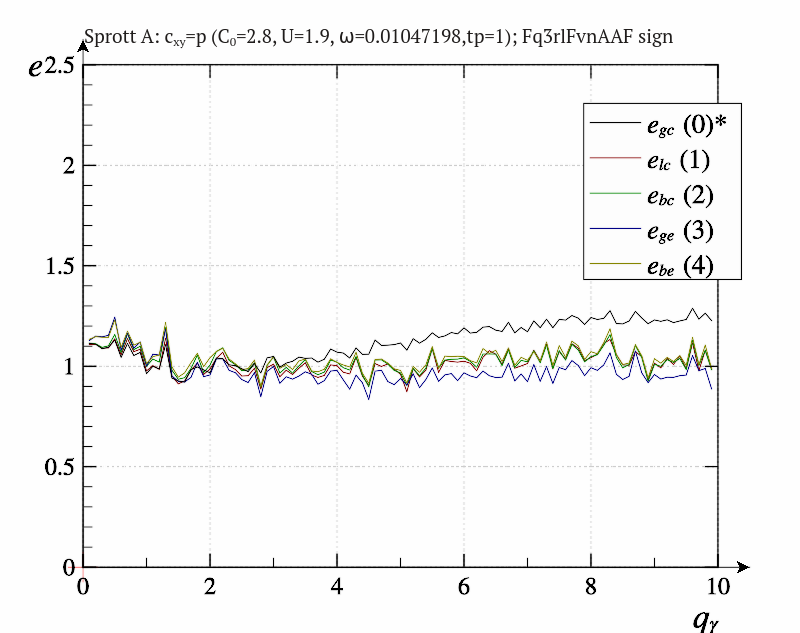
\includegraphics[width=0.49\textwidth]{p/cha/spr_a/Fq3rlFvnAAF_x2/sprott_a_id-p_q_gamma_sign.png}
    \hfill
    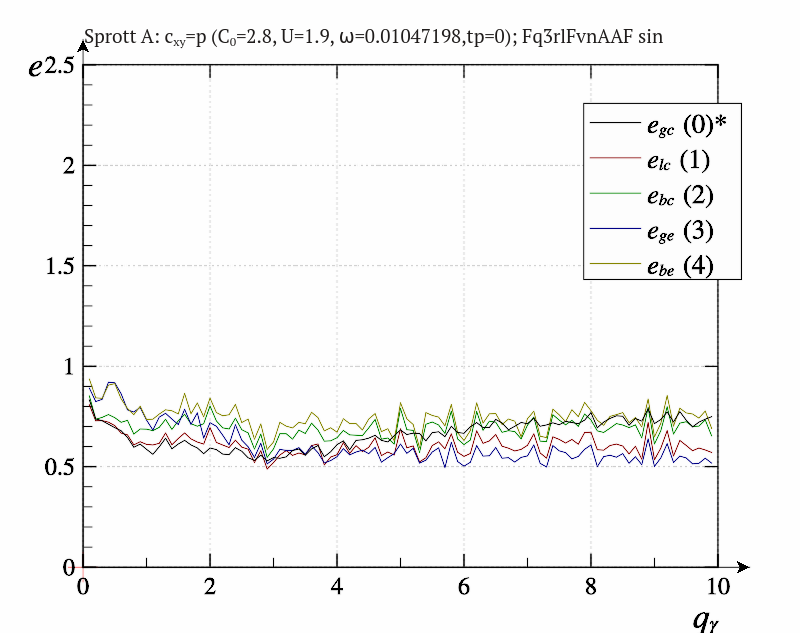
\includegraphics[width=0.49\textwidth]{p/cha/spr_a/Fq3rlFvnAAF_x2/sprott_a_id-p_q_gamma_sin.png}
  }
  \caption{Зависимости $\overline{e}(q_\gamma)$ при идентификации системы Sprott A группой методов Fq3rlFvnAAF.$q_{x^2}$
   при~(\ref{atu:eq:spr_a_po_t_sign}) и (\ref{atu:eq:spr_a_po_t_sin})}
  \label{atu:f:spr_a_qg_Fq3rlFvnAAF_q_x2}
\end{figure}

В целом, для данной системы
зависимости $\overline{e}( q_\gamma )$ % (рис.~\ref{atu:f:spr_a_e_qgamma})
свидетельствует о довольно слабом влиянии этого параметра
на динамику системы идентификации.
Проявляются робастные свойства поисковых агентов,
и для группы методов ql3rlWvnAAW эти свойства проявляются сильнее.



Рассмотрим влияние
параметра $v_f$, определяющий динамику поисковых агентов.


На рис.~\ref{atu:f:spr_a_v_f_ql3rlWvnAAW_q_x2} представлены зависимости
$\overline{e}(v_f)$ при применении группы методов ql3rlWvnAAW.$q_{x^2}$.
Зависимости практически нет. Это свидетельствует о том,
что смещение поисковых агентов в процессе поиска
для данной системы не имеет практически никакого смысла.
Скорее всего, это связано с тем, что в рассматриваемой постановке
время реакции системы на скачкообразные изменения параметра
имеет тот же порядок, что и требуемое время оценивания параметра,
что делает поиск практически бесполезным.
Рост ошибок идентификации на правом графике обусловлен
избыточной динамикой поисковых агентов.



\begin{figure}[htb!]
  \centerline{
    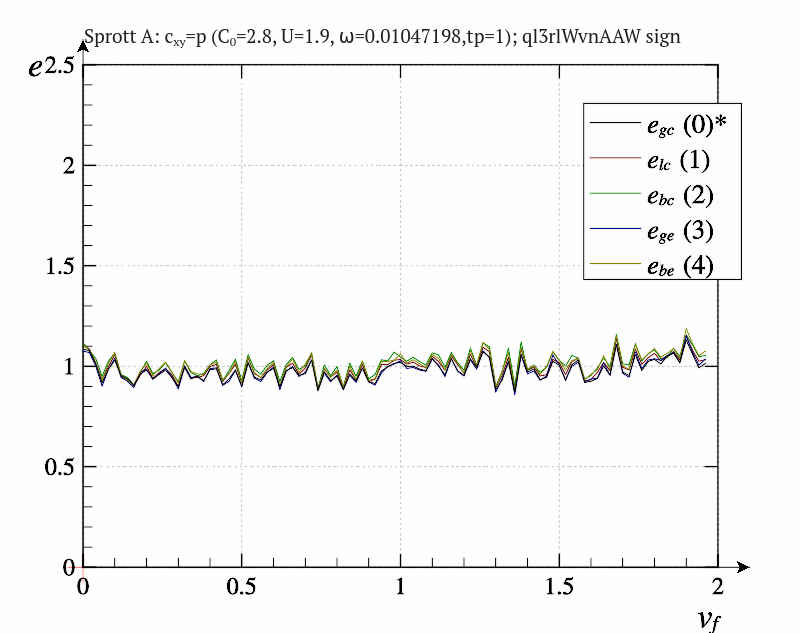
\includegraphics[width=0.49\textwidth]{p/cha/spr_a/ql3rlWvnAAW_x2/sprott_a_id-p_v_f_sign.png}
    \hfill
    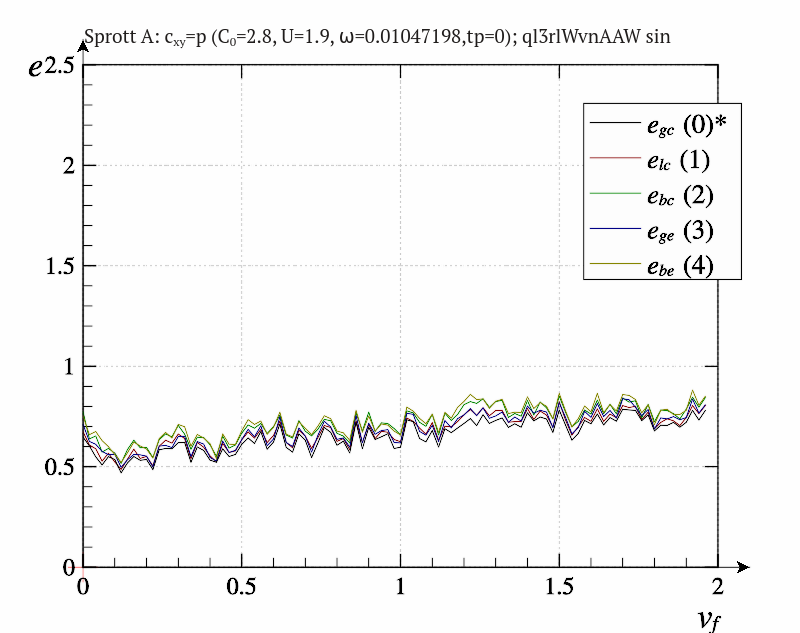
\includegraphics[width=0.49\textwidth]{p/cha/spr_a/ql3rlWvnAAW_x2/sprott_a_id-p_v_f_sin.png}
  }
  \caption{Зависимости $\overline{e}(v_f)$ при идентификации системы Sprott A группой методов ql3rlWvnAAW.$q_{x^2}$
   при~(\ref{atu:eq:spr_a_po_t_sign}) и (\ref{atu:eq:spr_a_po_t_sin})}
  \label{atu:f:spr_a_v_f_ql3rlWvnAAW_q_x2}
\end{figure}

На рис.~\ref{atu:f:spr_a_v_f_Fq3rlFvnAAF_q_x2} представлены зависимости
$\overline{e}(v_f)$ при применении методов Fq3rlFvnAAF.$q_{x^2}$.
Данные графики проявляют пусть незначительное,
но всё же заметное отличие от предыдущих.
Для этого метода существует слабо выраженный минимум,
причём для него $v_f \ne 0 $, что позволяет
оправдать применение поискового метода.

\begin{figure}[htb!]
  \centerline{
    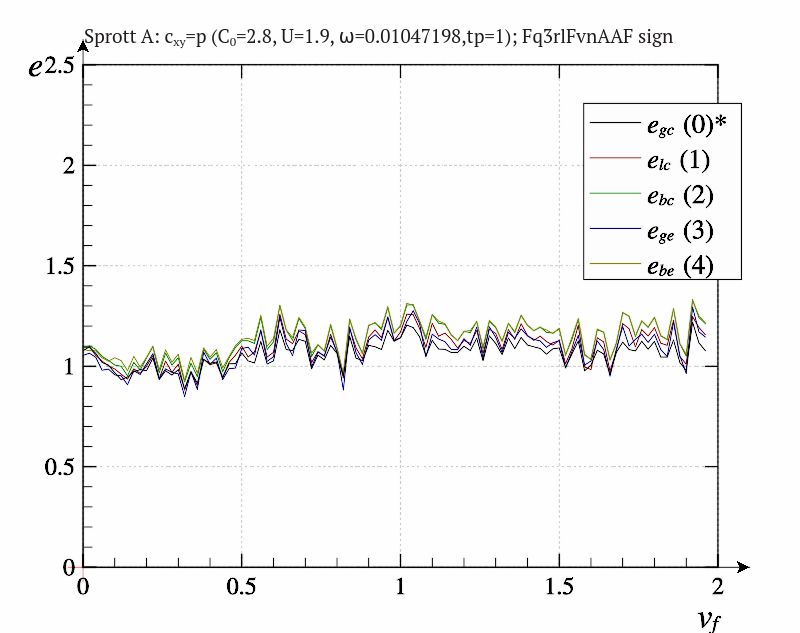
\includegraphics[width=0.49\textwidth]{p/cha/spr_a/Fq3rlFvnAAF_x2/sprott_a_id-p_v_f_sign.png}
    \hfill
    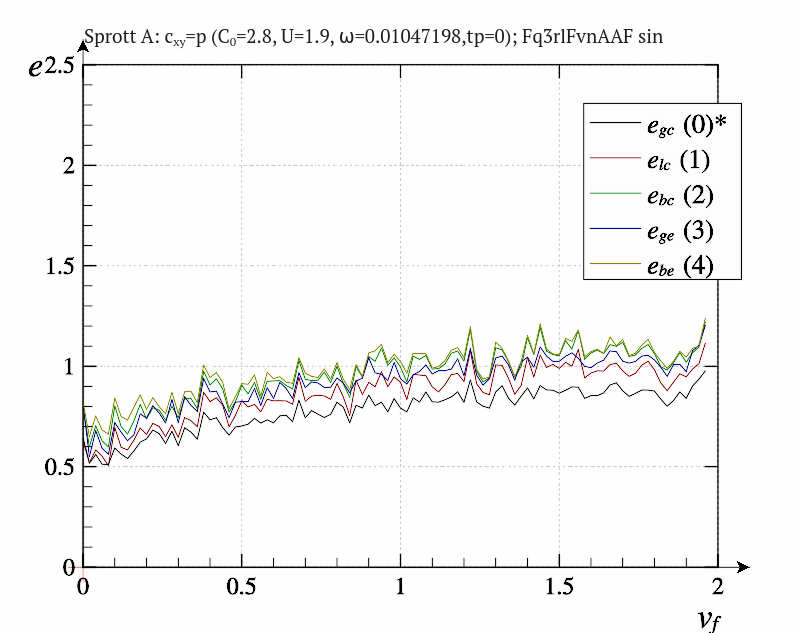
\includegraphics[width=0.49\textwidth]{p/cha/spr_a/Fq3rlFvnAAF_x2/sprott_a_id-p_v_f_sin.png}
  }
  \caption{Зависимости $\overline{e}(v_f)$ при идентификации системы Sprott A группой методов Fq3rlFvnAAF.$q_{x^2}$
   при~(\ref{atu:eq:spr_a_po_t_sign}) и (\ref{atu:eq:spr_a_po_t_sin})}
  \label{atu:f:spr_a_v_f_Fq3rlFvnAAF_q_x2}
\end{figure}

Параметр $k_e$, определяющий соотношение сил, действующих
на поисковый агент, для рассматриваемой системы не должен
иметь существенного влияния на процесс поиска.
Слабая зависимость от $v_f$ практически автоматически обозначает
и слабую зависимость от $k_e$, так как оба эти параметра
входят в определение одной и той же ``силы'',
определяющей смещение поисковых агентов, а из
анализа влияния предыдущего параметра было установлено,
что в данных конкретных условиях поиск практически не улучшает результаты.


На рис.~\ref{atu:f:spr_a_k_e_ql3rlWvnAAW_q_x2} представлены зависимости
$\overline{e}(k_e)$ при применении метода ql3rlWvnAAW.$q_{x^2}$.
Перемещение агентов в процессе поиска позволяет
уменьшить ошибку идентификации на 10--20\%.

\begin{figure}[htb!]
  \centerline{
    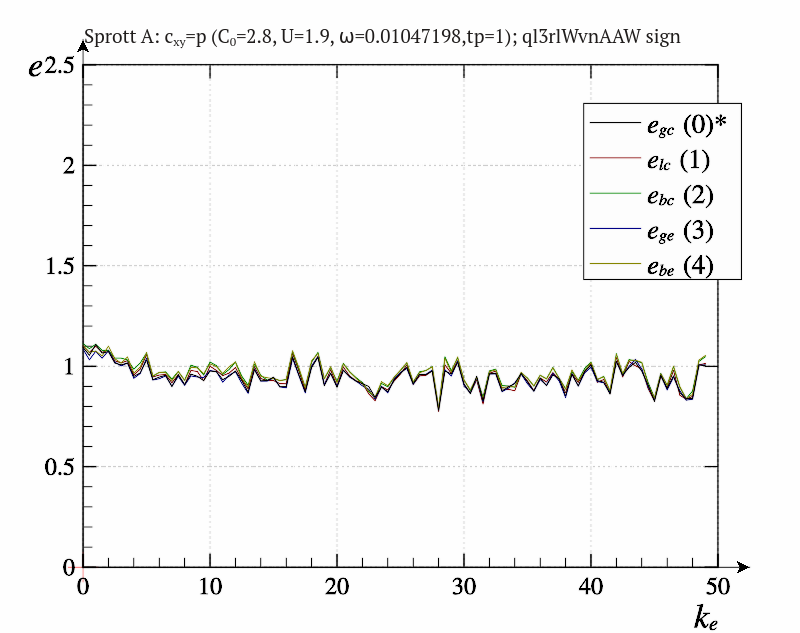
\includegraphics[width=0.49\textwidth]{p/cha/spr_a/ql3rlWvnAAW_x2/sprott_a_id-p_k_e_sign.png}
    \hfill
    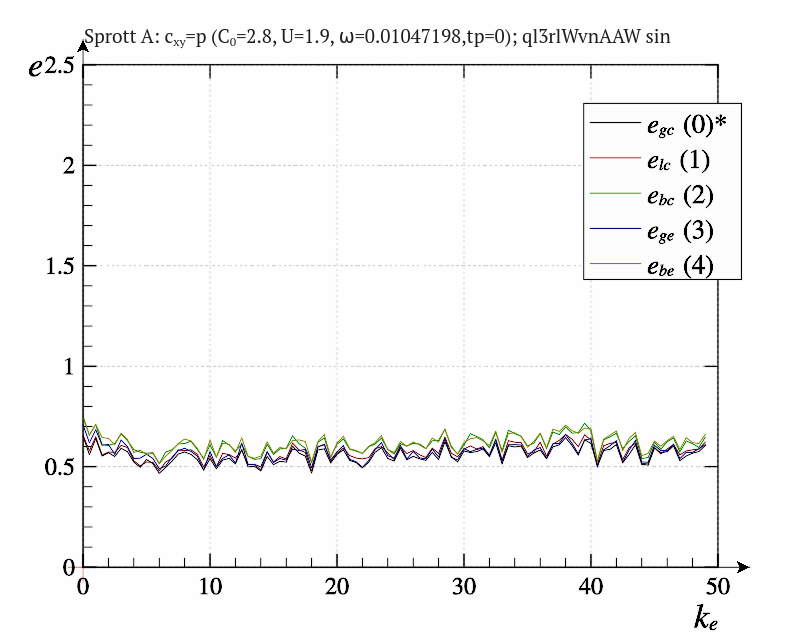
\includegraphics[width=0.49\textwidth]{p/cha/spr_a/ql3rlWvnAAW_x2/sprott_a_id-p_k_e_sin.png}
  }
  \caption{Зависимости $\overline{e}(k_e)$ при идентификации системы Sprott A группой методов ql3rlWvnAAW.$q_{x^2}$
   при~(\ref{atu:eq:spr_a_po_t_sign}) и (\ref{atu:eq:spr_a_po_t_sin})}
  \label{atu:f:spr_a_k_e_ql3rlWvnAAW_q_x2}
\end{figure}

На рис.~\ref{atu:f:spr_a_k_e_Fq3rlFvnAAF_q_x2} представлены зависимости
$\overline{e}(k_e)$ при применении методов Fq3rlFvnAAF.$q_{x^2}$.
В этом случае наблюдается рост ошибки идентификации при росте $k_e$
при условии~(\ref{atu:eq:spr_a_po_t_sin}). Динамика агентов при этом
становиться избыточной по сравнению с динамикой идентифицируемого параметра.

\begin{figure}[htb!]
  \centerline{
    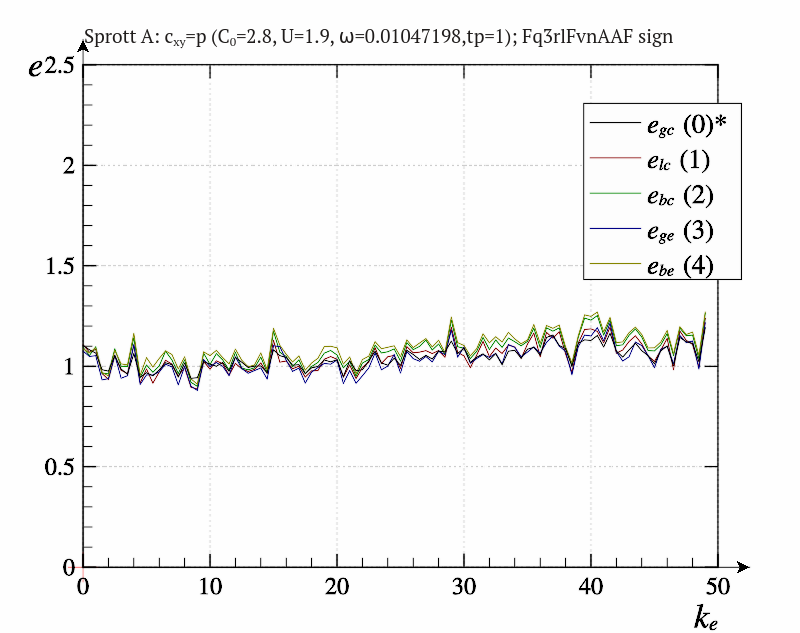
\includegraphics[width=0.49\textwidth]{p/cha/spr_a/Fq3rlFvnAAF_x2/sprott_a_id-p_k_e_sign.png}
    \hfill
    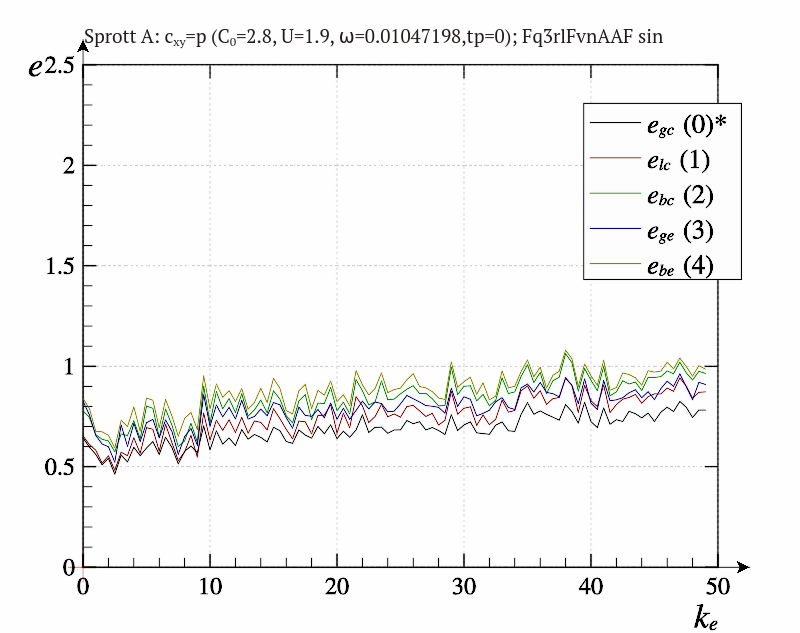
\includegraphics[width=0.49\textwidth]{p/cha/spr_a/Fq3rlFvnAAF_x2/sprott_a_id-p_k_e_sin.png}
  }
  \caption{Зависимости $\overline{e}(k_e)$ при идентификации системы Sprott A группой методов Fq3rlFvnAAF.$q_{x^2}$
   при~(\ref{atu:eq:spr_a_po_t_sign}) и (\ref{atu:eq:spr_a_po_t_sin})}
  \label{atu:f:spr_a_k_e_Fq3rlFvnAAF_q_x2}
\end{figure}

Как и ожидалось, зависимости $\overline{e}(k_e)$
довольно слабые, и аналогично зависимостям  $\overline{e}(v_f)$,
только для метода Fq3rlFvnAAF.$q_{x^2}$ можно
утверждать о необходимости поиска.

% }}}2

\subsection{Альтернативные критерии для системы Sprott A}   % {{{2

Представленные системы идентификации были основаны на критерии,
который были выбран путём перебора наиболее простых и очевидных кандидатов.
При этом удалось достичь работоспособности систем,
однако, ошибки идентификации были весьма высоки.
Следовательно, имеет смысл создать и использовать другие критерии,
используя больше информации о системе.

В первую очередь, сравнивая зависимости $q_{x^2}(c_{x_y})$ и $q_{y^2}(c_{x_y})$
(рис.~\ref{atu:f:spr_a_q}), можно заметить, что
пики и провалы этих зависимостей близки, а  $q_{y^2}(c_{x_y})$
в целом практически не зависит от $c_{x_y}$.
Таким образом, можно использовать критерий вида
%
\[
  q_{x2Oy2} = \frac{q_{x^2}}{q_{y^2}}.
\]

Далее, исходя из вида первого из уравнений системы~(\ref{atu:eq:spr_a})
можно сделать вывод о том, что величина
%
\begin{equation}
  q_{dxOy} =
  \frac{\overline{\dot{x}y}}{\overline{\dot{x}^2}}
  \label{atu:eq:spr_a_q_dxyOdx2}
\end{equation}
%
может быть использована в качестве критерия с широким рабочим диапазоном.
Под знаком усреднения подразумевается или скользящее среднее,
или же экспоненциальное сглаживание.
Существенным недостатком данного критерия является использование
производных, которые как из-за реальных ошибок измерения $x(t)$,
та и и-за ошибок оценивания производной подвержены
скачкам большой амплитуды. Это ограничивает применимость данного критерия
значительными интервалами оценивания, т.е. малыми величинами $a_q$.

Вид зависимостей для критериев $q_{x2Oy2}$ и $q_{dxOy}$,
в сравнении с критериями $q_{x^2}$ и $q_{y^2}$
представлены на  рис.~\ref{atu:f:spr_a_q_alt}.

\begin{figure}[htb!]
\centerline{
  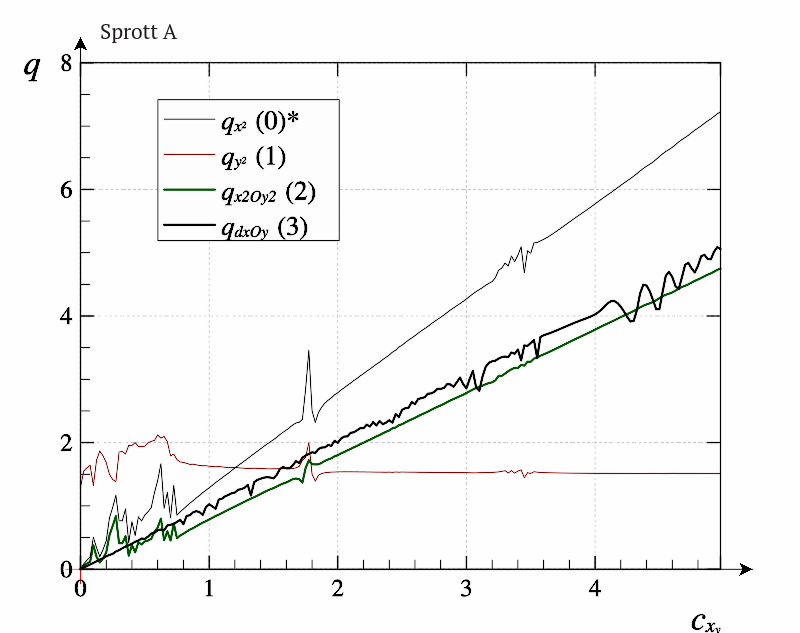
\includegraphics[width=0.60\textwidth]{p/cha/spr_a/sprott_a_q2-p_c_x_y2.png}
}
\caption{Зависимости альтернативных критериев $q(c_{x_y})$ для системы (\ref{atu:eq:spr_a}) }
\label{atu:f:spr_a_q_alt}
\end{figure}

Анализ этих зависимостей позволяет сделать вывод о том,
что критерий $q_{x2Oy2}$ характеризуется
значительно меньшими возмущениями, тем исходный  $q_{x^2}$,
однако эти возмущения всё же есть. При этом сохраняется
начальный участок с сильным нарушением монотонности.
Критерий $q_{dxOy}$ напротив, несмотря на возмущения,
характеризуется зависимостью, более близкой к линейной,
при этом она сохраняется как на начальном участке,
так и в областях импульсных возмущений других критериев.
Следовательно, этот критерий имеет смысл использовать
при создании системы идентификации.

Рассмотрим процесс идентификации при условиях~(\ref{atu:eq:spr_a_po_t_sign})
при использовании группы методов ql3rlWvnAAW.$q_{dxOy}$.
Результаты моделирования приведены на рис.~\ref{atu:f:spr_a_id_ql3rlWvnAAW_q_dxOy_sign}.

\begin{figure}[htb!]
  \centerline{
    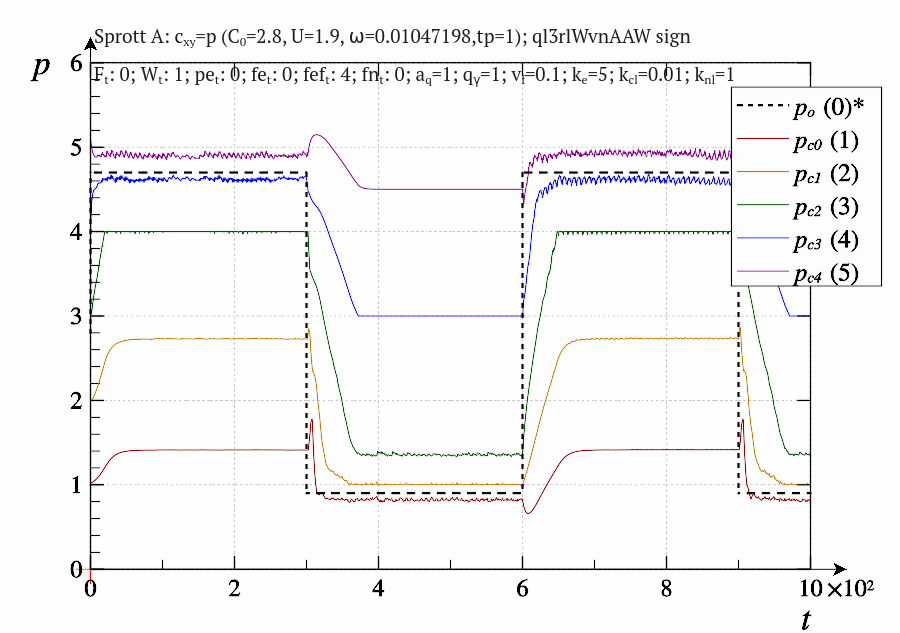
\includegraphics[width=0.49\textwidth]{p/cha/spr_a/ql3rlWvnAAW_dxOy/sprott_a_id2-p_t_pi_ql3rlWvnAAW_sign.png}
    \hfill
    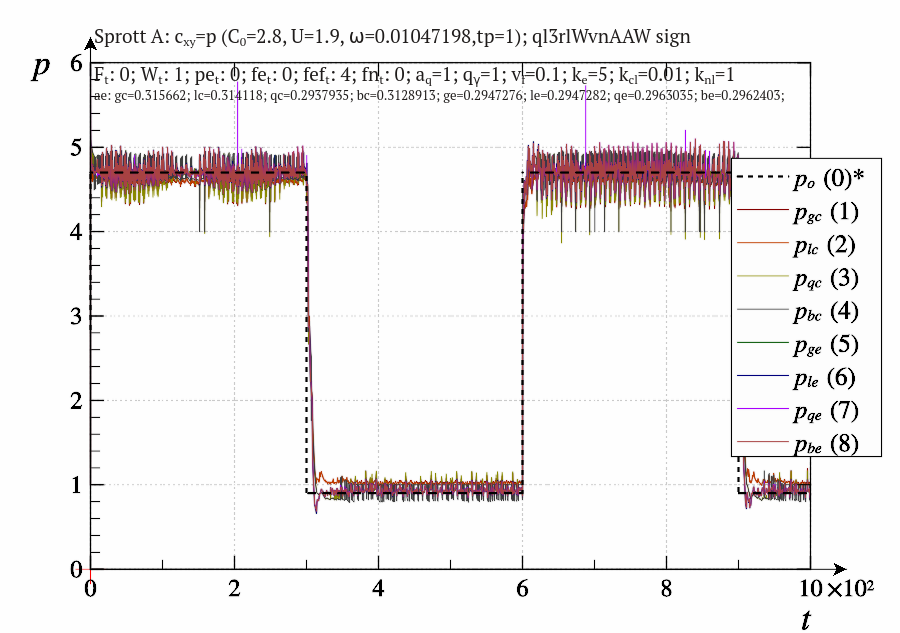
\includegraphics[width=0.49\textwidth]{p/cha/spr_a/ql3rlWvnAAW_dxOy/sprott_a_id2-p_t_p_ql3rlWvnAAW_sign.png}
  }
  \caption{Процесс идентификации параметра ``$c_{x_y}$'' системы Sprott A группой методов ql3rlWvnAAW.$q_{dxOy}$ при условии~(\ref{atu:eq:spr_a_po_t_sign})}
  \label{atu:f:spr_a_id_ql3rlWvnAAW_q_dxOy_sign}
\end{figure}

Сравнивая эти результатов с теми, что были приведены на рис.~\ref{atu:f:spr_a_id_ql3rlWvnAAW_q_x2_sign},
можно отметить, что несмотря на сохранившиеся высокочастотные колебания,
уровень ошибки идентификации существенно уменьшился.

Результаты моделирования для этого же метода,
но при условии~(\ref{atu:eq:spr_a_po_t_sin}) приведены на рис.~\ref{atu:f:spr_a_id_ql3rlWvnAAW_q_dxOy_sin}.
В отличие от методов с применением критерия $q_{x^2}$,
здесь переход к плавному изменению идентифицируемого параметра приводит
к значительному снижению уровня ошибки. Не только
уменьшился размах колебаний, но и систематические ошибки стали значительно меньше.
Также существенно снизилось время реакции на изменение параметра.

\begin{figure}[htb!]
  \centerline{
    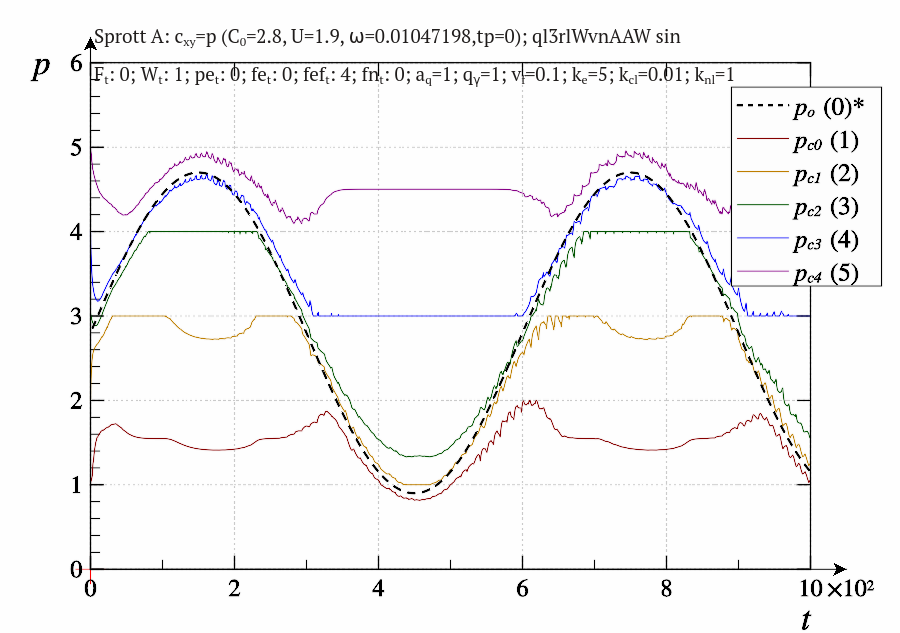
\includegraphics[width=0.49\textwidth]{p/cha/spr_a/ql3rlWvnAAW_dxOy/sprott_a_id2-p_t_pi_ql3rlWvnAAW_sin.png}
    \hfill
    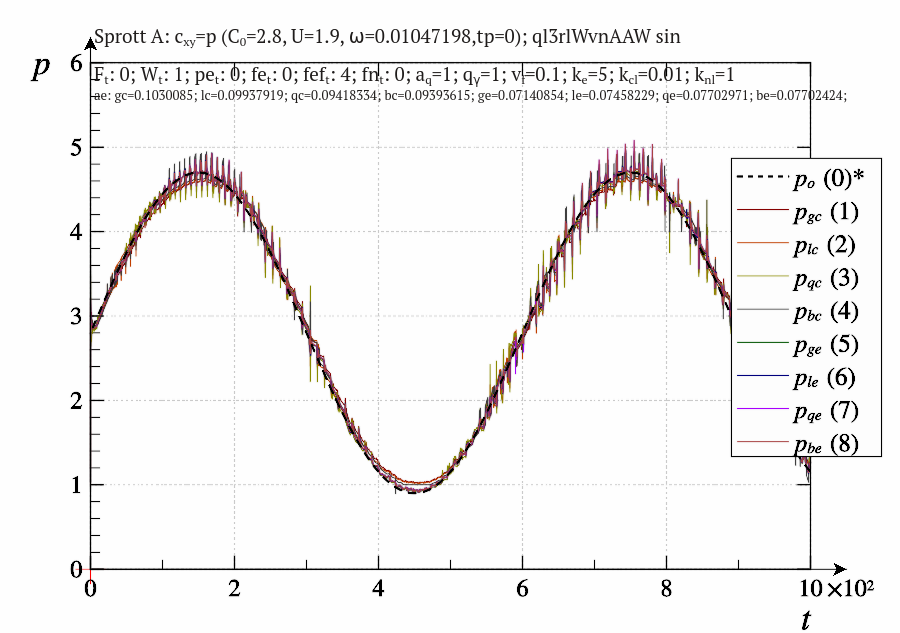
\includegraphics[width=0.49\textwidth]{p/cha/spr_a/ql3rlWvnAAW_dxOy/sprott_a_id2-p_t_p_ql3rlWvnAAW_sin.png}
  }
  \caption{Процесс идентификации параметра ``$c_{x_y}$'' системы Sprott A группой методов ql3rlWvnAAW.$q_{dxOy}$ при условии~(\ref{atu:eq:spr_a_po_t_sin})}
  \label{atu:f:spr_a_id_ql3rlWvnAAW_q_dxOy_sin}
\end{figure}

Для проверки равномерности идентификации от значения параметра
рассмотрим процесс идентификации при условии~(\ref{atu:eq:po_t_ramp})
(рис.~\ref{atu:f:spr_a_id_ql3rlWvnAAW_q_dxOy_ramp}).

\begin{figure}[htb!]
  \centerline{
    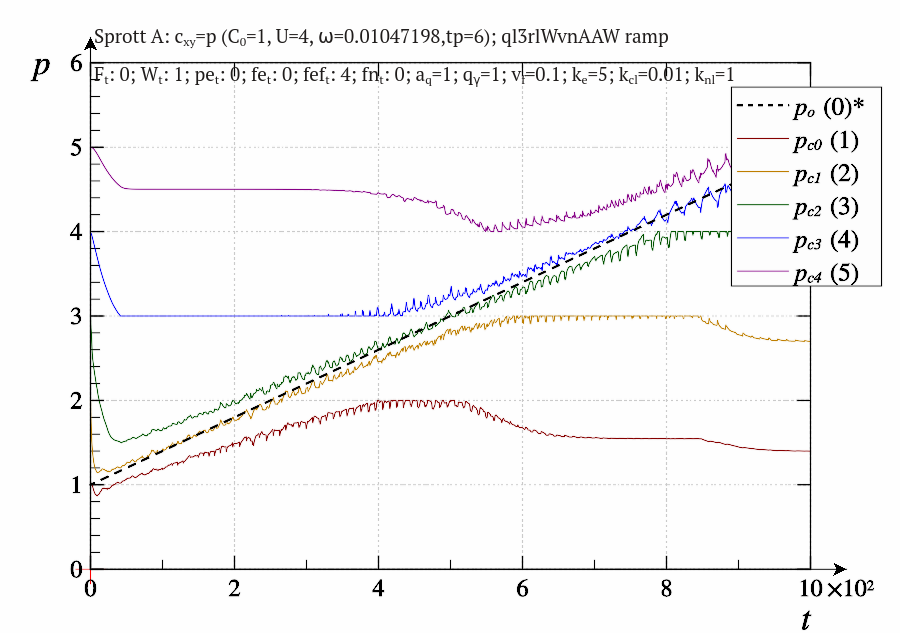
\includegraphics[width=0.49\textwidth]{p/cha/spr_a/ql3rlWvnAAW_dxOy/sprott_a_id2-p_t_pi_ql3rlWvnAAW_ramp.png}
    \hfill
    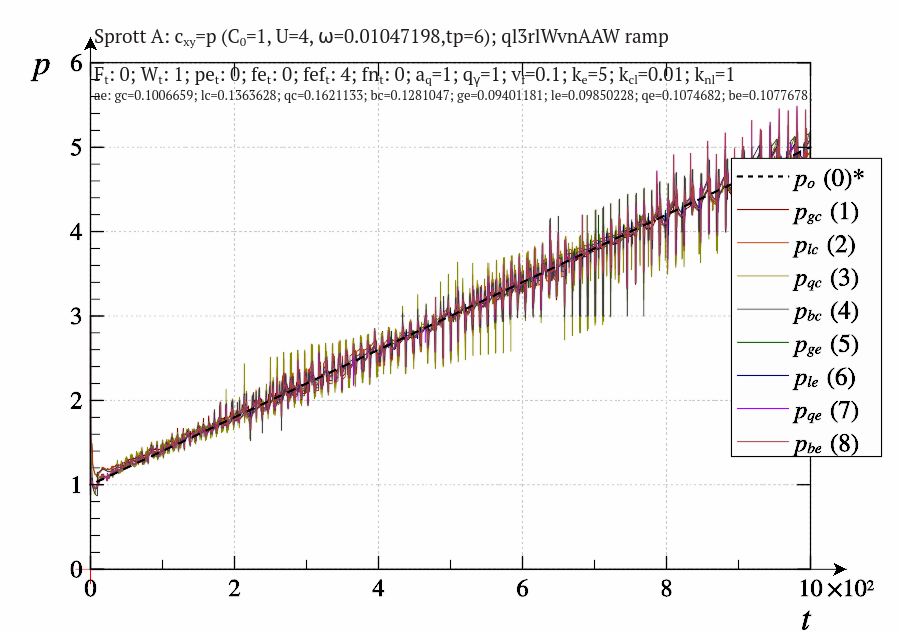
\includegraphics[width=0.49\textwidth]{p/cha/spr_a/ql3rlWvnAAW_dxOy/sprott_a_id2-p_t_p_ql3rlWvnAAW_ramp.png}
  }
  \caption{Процесс идентификации параметра ``$c_{x_y}$'' системы Sprott A группой методов ql3rlWvnAAW.$q_{dxOy}$ при условии~(\ref{atu:eq:po_t_ramp})}
  \label{atu:f:spr_a_id_ql3rlWvnAAW_q_dxOy_ramp}
\end{figure}

При сравнении с результатами, приведёнными на рис.~\ref{atu:f:spr_a_id_ql3rlWvnAAW_q_x2_ramp},
можно сделать вывод о том, что во всём диапазоне изменения параметра
не наблюдается заметных отклонений $p_\mathrm{id}$ от $p_o$,
если не учитывать высокочастотные возмущения. Выход на рабочий режим также проиходит быстрее.
Однако, имульсные возмущения всё равно присутствуют,
хотя и в меньшей степени.

На рис.~\ref{atu:f:spr_a_a_q_ql3rlWvnAAW_q_dxOy} представлены зависимости
$\overline{e}(a_q)$ при применении метода ql3rlWvnAAW.$q_{dxOy}$.
Наблюдается как общее существенно снижения урвня ошибки идентификации,
так обоснованное разделение этого уровня от метода
координатора поиска при условии~(\ref{atu:eq:spr_a_po_t_sin}).
Ошибка при использовании метода $p_{gc}$ ограничена снизу
из-за влияния агентов, расположенных в удалении от $p_o$.

\begin{figure}[htb!]
  \centerline{
    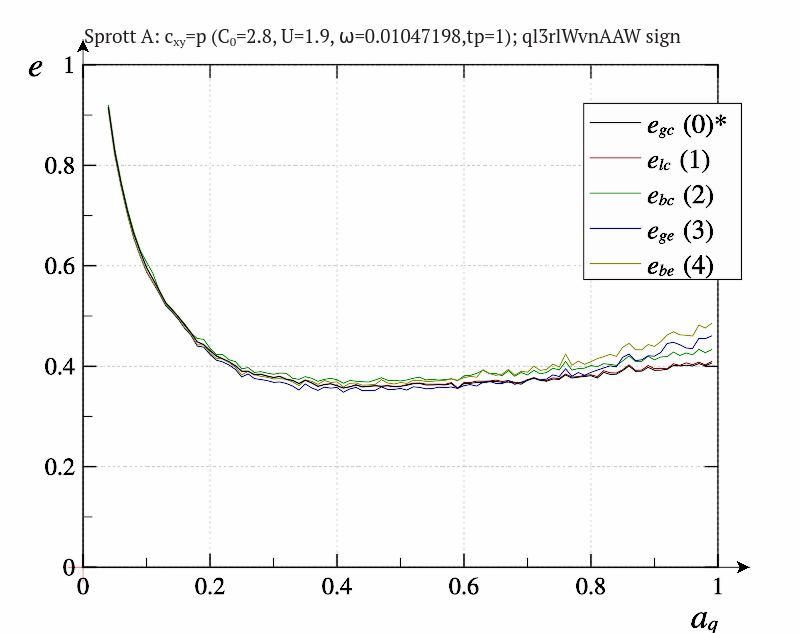
\includegraphics[width=0.49\textwidth]{p/cha/spr_a/ql3rlWvnAAW_dxOy/sprott_a_id2-p_a_q_sign.png}
    \hfill
    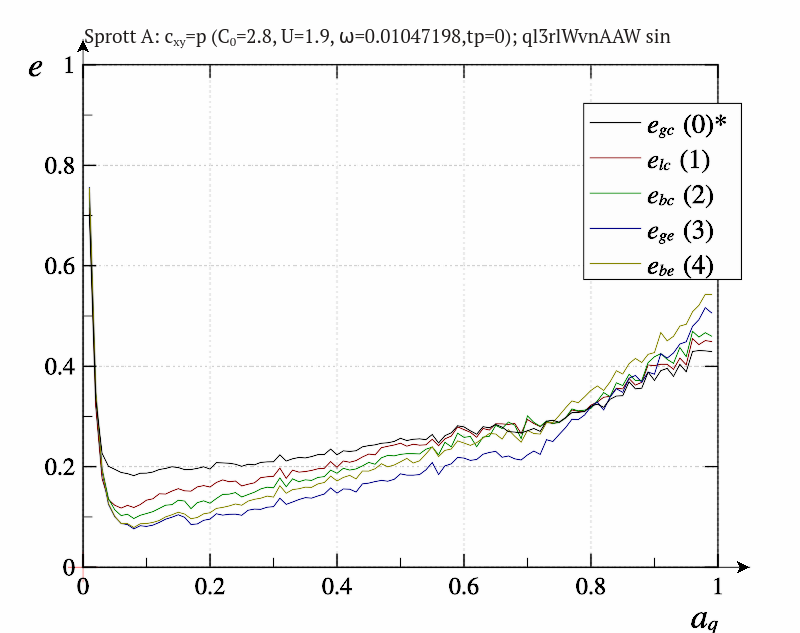
\includegraphics[width=0.49\textwidth]{p/cha/spr_a/ql3rlWvnAAW_dxOy/sprott_a_id2-p_a_q_sin.png}
  }
  \caption{Зависимости $\overline{e}(a_q)$ при идентификации системы Sprott A группой методов ql3rlWvnAAW.$q_{dxOy}$
   при~(\ref{atu:eq:spr_a_po_t_sign}) и (\ref{atu:eq:spr_a_po_t_sin})}
  \label{atu:f:spr_a_a_q_ql3rlWvnAAW_q_dxOy}
\end{figure}

На рис.~\ref{atu:f:spr_a_ql3rlWvnAAW_q_dxOy} представлены зависимости
$\overline{e}(q_\gamma)$ при применении группы методов ql3rlWvnAAW.$q_{dxOy}$.

\begin{figure}[htb!]
  \centerline{
    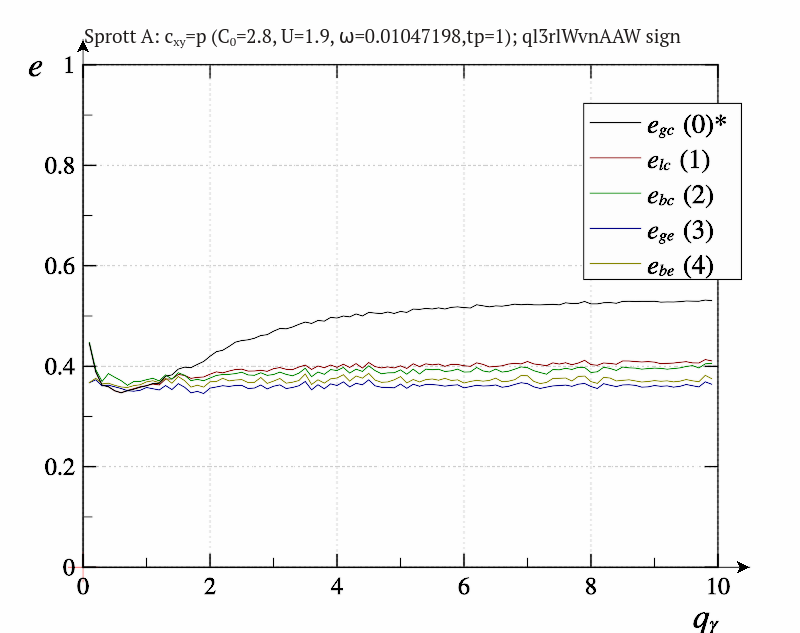
\includegraphics[width=0.49\textwidth]{p/cha/spr_a/ql3rlWvnAAW_dxOy/sprott_a_id2-p_q_gamma_sign.png}
    \hfill
    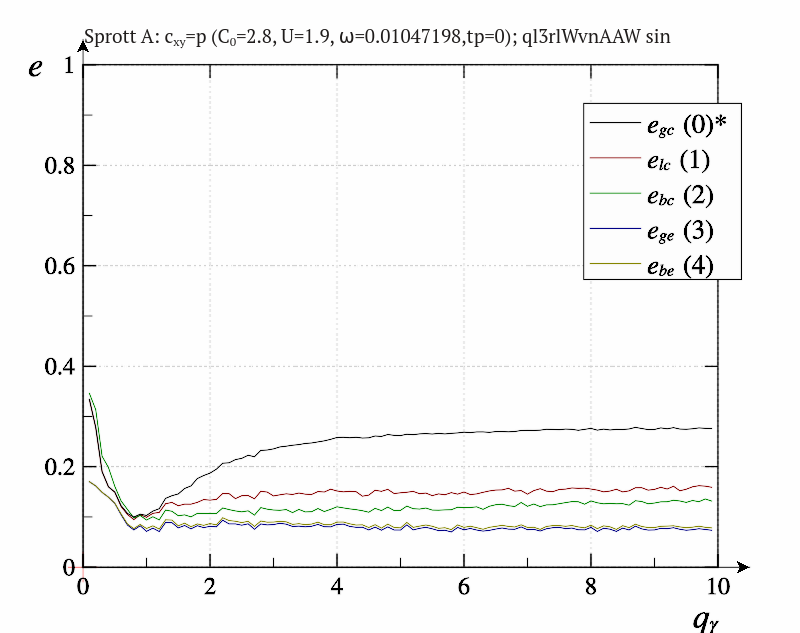
\includegraphics[width=0.49\textwidth]{p/cha/spr_a/ql3rlWvnAAW_dxOy/sprott_a_id2-p_q_gamma_sin.png}
  }
  \caption{Зависимости $\overline{e}(q_\gamma)$ при идентификации системы Sprott A группой методов ql3rlWvnAAW.$q_{dxOy}$
   при~(\ref{atu:eq:spr_a_po_t_sign}) и (\ref{atu:eq:spr_a_po_t_sin})}
  \label{atu:f:spr_a_ql3rlWvnAAW_q_dxOy}
\end{figure}

Существенно меньший уровень ошибок идентификации,
про сравнению с результатами, приведёнными на рис.~\ref{atu:f:spr_a_qg_Fq3rlFvnAAF_q_x2}
позволяет более чётко проявить влияние параметра $q_\gamma$.
Явно выражен рост ошибки для всех методов координатора при избыточной
чувствительности, а также слабую зависимость для большинства методов
за пределами этой зоны. Исключение составляет метод $p_{gc}$,
который и должен быть наиболее подверженным влиянию
недостаточной чувствительности функции качества.

На рис.~\ref{atu:f:spr_a_v_f_ql3rlWvnAAW_q_dxOy} представлены зависимости
$\overline{e}(v_f)$ при применении группы методов ql3rlWvnAAW.$q_{dxOy}$.
Если при использовании критерия $q_{x^2}$ зависимость была по большей части условной,
то в данном случае, особенно при условии  (\ref{atu:eq:spr_a_po_t_sin}),
динамика агентов даёт существенный вклад, уменьшая ошибку идентификации в 2--3 раза.

\begin{figure}[htb!]
  \centerline{
    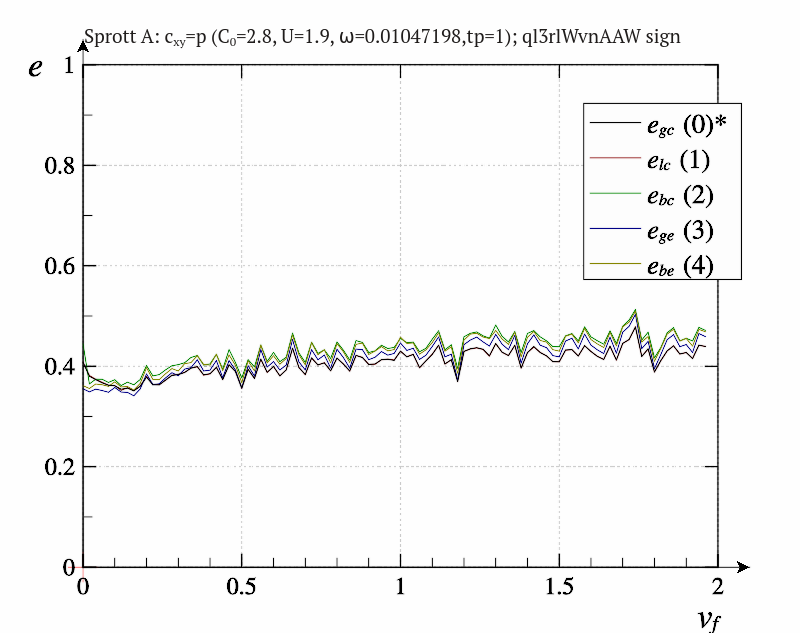
\includegraphics[width=0.49\textwidth]{p/cha/spr_a/ql3rlWvnAAW_dxOy/sprott_a_id2-p_v_f_sign.png}
    \hfill
    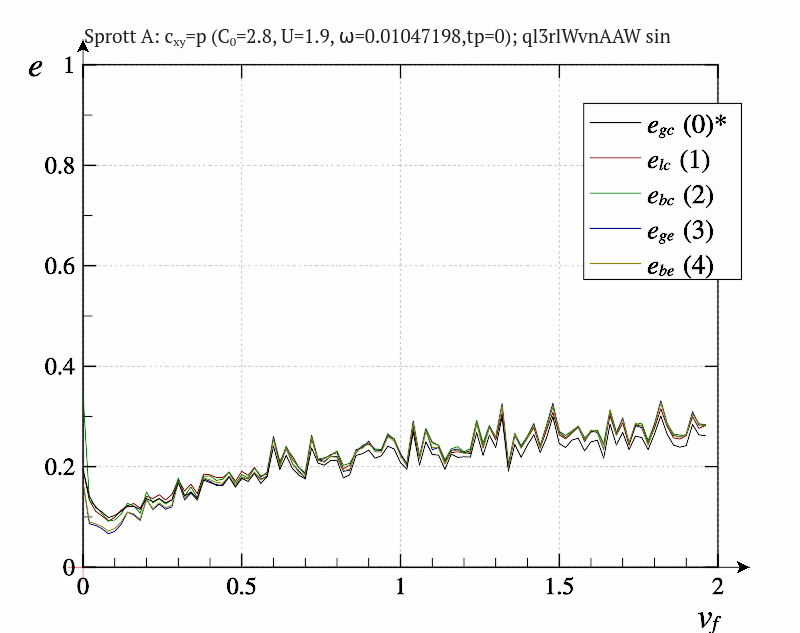
\includegraphics[width=0.49\textwidth]{p/cha/spr_a/ql3rlWvnAAW_dxOy/sprott_a_id2-p_v_f_sin.png}
  }
  \caption{Зависимости $\overline{e}(v_f)$ при идентификации системы Sprott A группой методов ql3rlWvnAAW.$q_{dxOy}$
   при~(\ref{atu:eq:spr_a_po_t_sign}) и (\ref{atu:eq:spr_a_po_t_sin})}
  \label{atu:f:spr_a_v_f_ql3rlWvnAAW_q_dxOy}
\end{figure}

Таким образом, использование критерия $q_{dxOy}$
позволяет повысить точность идентификации при всех рассмотренных
условиях. Недостатком является большие вычислительные затраты
на вычисление данного критерия, но в большинстве случаев это не является проблемой.


% }}}2

\subsection{Выводы}  % {{{2

В целом, результаты моделирования процессов идентификации системы ``Sprott A'',
и сравнение этих результатов, с данными, полученными
для системы Лоренца, позволяют сделать следующие выводы:

\begin{itemize}

  \item
    Попытка создать и критерий идентификации и работоспособную систему идентификации
    на основании энергетического критерия вида $q_{x^2}$ оказалась успешной.
    Однако уровень ошибок идентификации при этом не позволяет
    заметно улучшить качество идентификации за счёт настройки её параметров.

  \item
    Использование критерия $q_{dxOy}$ даёт существенно лучшие результаты,
    и появляется возможность успешно настраивать систему идентификации.

  \item
    Все рассмотренные критерии подвержены импульсным возмущениям,
    что приводи к высокочастотным колебаниям значения $p_{\mathrm{id}}$.

  \item
    В целом, использование метода  ql3rlWvnleW.$q_{x^2}$ для данной системы
    и начальных условий наиболее оправданно.

\end{itemize}

% }}}2


% }}}1

% vim: fdm=marker foldlevel=1 foldignore="%#" fdc=4 ft=tex
